\documentclass[12pt, atypical, journal]{article}

\usepackage[utf8]{inputenc}
\usepackage[spanish,es-tabla]{babel}
\usepackage{geometry}
\geometry{letterpaper, margin=2.54cm}
\usepackage{times}
\usepackage{setspace}
\onehalfspacing
\usepackage{graphicx}
\usepackage{booktabs}
\usepackage{longtable}
\usepackage{titlesec}
\usepackage{hyperref}
\usepackage{caption}

\newenvironment{hangparas}[2]{\setlength{\parindent}{-#1}\setlength{\leftmargin}{#1}\everypar{\hangindent=#1}}{\par}

\hypersetup{
   colorlinks=true,
   linkcolor=black,
   filecolor=black,     
   urlcolor=blue,
   citecolor=black
}

\titleformat{\section}{\normalfont\Large\bfseries}{\thesection.}{0.5em}{}
\titleformat{\subsection}{\normalfont\large\bfseries}{\thesubsection.}{0.5em}{}
\titleformat{\subsubsection}{\normalfont\normalsize\bfseries\itshape}{\thesubsubsection.}{0.5em}{}

\usepackage{pdfpages}
\usepackage{float}
\usepackage{listings}
\usepackage{xcolor}
\lstset{
    basicstyle=\ttfamily\footnotesize,
    breaklines=true,
    frame=single,
    showstringspaces=false,
    tabsize=2,
    extendedchars=true,
    literate={á}{{\'a}}1 {é}{{\'e}}1 {í}{{\'i}}1 {ó}{{\'o}}1 {ú}{{\'u}}1 {Á}{{\'A}}1 {É}{{\'E}}1 {Í}{{\'I}}1 {Ó}{{\'O}}1 {Ú}{{\'U}}1 {ñ}{{\~n}}1 {Ñ}{{\~N}}1
}

\begin{document}

% ==============================================================================
% 1. PORTADA
% ==============================================================================
\begin{titlepage}
   \begin{center}
       \vspace*{1cm}
      
       {\Large\bfseries UNIVERSIDAD POLITÉCNICA DE CHIAPAS} \\[0.5cm]
       {\large\bfseries INGENIERÍA EN TECNOLOGÍAS DE LA INFORMACIÓN E INNOVACIÓN DIGITAL} \\[1.5cm]
      
       \vfill
      
       {\Large\bfseries REPORTE DE PROYECTO INTEGRADOR II} \\[1cm]
      
       \textbf{Nombre del Proyecto:} \\
       \textbf{Nombre del Proyecto:} \\
       {\large LecturaMétrica: Plataforma Web para la Gestión Automatizada, Analítica y Gamificada del Hábito Lector} \\[1.5cm]
      
       \vfill
      
       \textbf{Integrantes del Equipo:} \\[0.3cm]
       {\large Patricia Alejandra Clemente Chacón (Matrícula: 251237)} \\
       {\large Nínive Argelia Pérez González (Matrícula: 251239)} \\
       {\large Mónica Jamileth Velázquez García (Matrícula: 243729)} \\[1.5cm]
      
       \textbf{Docente:} \\
       {\large Hernandez Camacho Rocio Crystal} \\[1.5cm]
      
       \vfill
      
       \textbf{Fecha de entrega:} \\
       {\large 26 de junio de 2026}
      
       \vspace*{1cm}
   \end{center}
\end{titlepage}

\newpage

% ==============================================================================
% ÍNDICES
% ==============================================================================
\tableofcontents
\newpage

\listoffigures
\newpage

\listoftables
\newpage

% ==============================================================================
% 2. RESUMEN
% ==============================================================================
\section{Resumen}

Este proyecto presenta el desarrollo de una aplicación web dedicada a la lectura métrica y la optimización de procesos mediante la recopilación, almacenamiento y visualización de indicadores clave de rendimiento. El sistema fue concebido para mitigar los errores derivados del registro manual y solucionar la falta de centralización de la información en entornos organizacionales.

Arquitectónicamente, el desarrollo se basa en una estructura modular y desacoplada que garantiza la escalabilidad y mantenibilidad del sistema. El \textit{frontend}, construido con Next.js y React, proporciona una interfaz de usuario reactiva y optimizada mediante Tailwind CSS, mientras que el \textit{backend} implementa una arquitectura limpia (\textit{Clean Architecture}) utilizando Java, Spring Boot y Hibernate. Este diseño permite una clara separación entre la lógica de negocio y la infraestructura, apoyándose en PostgreSQL para asegurar la integridad y persistencia de los datos.

\vspace{0.5cm}
\noindent \textbf{Palabras clave:} Aplicación Web, Hábitos de Lectura, Seguimiento, Arquitectura Limpia.

% ==============================================================================
% 3. INTRODUCCIÓN
% ==============================================================================
\section{Introducción}

\subsection{Breve explicación del entorno del problema}
Muchas personas enfrentan dificultades para mantener un hábito de lectura constante debido a que llevar un control manual de su avance resulta tedioso y poco práctico. Por un lado, los lectores principiantes suelen desmotivarse al no ver su progreso de forma clara; por otro lado, los lectores habituales carecen de una herramienta centralizada para organizar libros y volúmenes con muchos capítulos. Esta falta de seguimiento provoca que la lectura se vuelva desorganizada y sea fácil de abandonar.

\subsection{Importancia del desarrollo}
Este proyecto se centra en desarrollar la aplicación web \textbf{LecturaMétrica} para facilitar el seguimiento y la organización de la lectura personal. La importancia del sistema radica en eliminar el esfuerzo de llevar bitácoras manuales, ofreciendo a los usuarios un registro automático de su avance. Al integrar dinámicas de motivación —como el control de rachas continuas e insignias— y un espacio de intercambio literario, la plataforma busca motivar a las personas a leer con mayor constancia y a comprender mejor sus hábitos mediante estadísticas claras.

\subsection{Alcances y limitaciones}
El alcance del proyecto contempla el desarrollo de funcionalidades básicas para la gestión de cuentas de usuario, una biblioteca personal para catalogar obras, un temporizador para cronometrar las sesiones de lectura, un tablero de estadísticas y un buzón para intercambiar recomendaciones literarias entre usuarios. Como limitaciones, el sistema no almacena ni visualiza archivos de libros digitales (como PDF o EPUB) por cuestiones de derechos de autor, ni incluye salas de chat públicas en tiempo real.

\subsection{Estructura del documento}
Este documento está organizado en secciones secuenciales que cubren todo el ciclo de desarrollo del proyecto. En sus capítulos se incluye el planteamiento y análisis del problema, la definición de objetivos, el marco teórico y normativo, así como el diseño arquitectónico, la implementación y las pruebas funcionales del sistema.

\newpage

% ==============================================================================
% 4. PLANTEAMIENTO DEL PROBLEMA
% ==============================================================================
\section{Planteamiento del problema}

\subsection{Descripción del problema en su contexto}
En la actualidad, muchas personas que desean desarrollar o mantener el hábito de la lectura se enfrentan a la falta de herramientas accesibles para cuantificar su rendimiento diario. En el contexto cotidiano, los lectores se dividen en dos grupos principales que experimentan dificultades similares: por un lado, los lectores principiantes sufren de desmotivación y abandono prematuro al sentir que leer es una actividad aislada y difícil de medir; por otro lado, los lectores habituales —que consumen libros, mangas o novelas gráficas— carecen de un espacio centralizado para organizar grandes volúmenes de capítulos. Al depender de bitácoras manuales o notas dispersas, el control del avance se vuelve una tarea tediosa que termina por interrumpir la constancia del usuario.

\subsection{Antecedentes y evidencia}
Las herramientas existentes en el mercado presentan un vacío operativo significativo. Por una parte, existen redes sociales abiertas orientadas a la publicación de textos (como Wattpad o Webtoon) que no ofrecen herramientas métricas personales; por otra parte, plataformas de catálogo literario (como Goodreads) o plantillas de hojas de cálculo (Excel) dependen de un llenado manual repetitivo. Experiencias y estudios de usabilidad en aplicaciones de registro de hábitos demuestran que la alta fricción operativa —es decir, la pérdida de tiempo y el esfuerzo cognitivo que implica registrar datos a mano— es la causa primordial por la cual los usuarios abandonan el uso de estas herramientas durante las primeras semanas, generando frustración e interrumpiendo su ciclo de lectura.

\subsection{Declaración clara del problema}
El problema identificado es la ausencia de un sistema web accesible, centralizado y automatizado que permita a los lectores cuantificar su avance en tiempo real, lo que ocasiona la pérdida del hábito lector en usuarios novatos debido a la pesadez del registro manual, y la desorganización de la biblioteca personal en lectores avanzados al carecer de una herramienta unificada para gestionar sus estadísticas.

\subsection{Consecuencias del problema}
De no resolver esta situación, los usuarios continuarán perdiendo el hábito y la disciplina de lectura al no contar con estímulos constantes ni visibilidad sobre su propio progreso. Las repercusiones inmediatas incluyen la falta de organización de las bibliotecas personales, la pérdida del historial de avance en lecturas largas y la imposibilidad de conocer el ritmo real de lectura. A largo plazo, esta desorganización desmotiva al usuario y limita el desarrollo de habilidades cognitivas, académicas y de concentración ligadas a la lectura diaria.

\subsection{Delimitación del problema}
Este proyecto se delimita estrictamente al desarrollo de una plataforma web para la recolección, automatización y análisis de métricas individuales de lectura. El sistema procesará metadatos, tiempos de lectura, páginas y micro-reseñas en texto plano escritas por los propios usuarios. No se incluirá el soporte para procesamiento de archivos de lectura digital, la captura de imágenes de obras externas, ni funciones de interacción social síncrona o perfiles públicos abiertos.

\subsection{Preguntas de investigación}
Para guiar el desarrollo de la solución propuesta, se plantean las siguientes interrogantes clave:
\begin{enumerate}
    \item ¿Cómo diseñar un sistema web que automatice el registro de obras y cronometre las sesiones de lectura para eliminar la carga del llenado manual en los usuarios?
    \item ¿De qué manera influye la integración de mecánicas de gamificación y de un buzón de intercambio literario asíncrono en la constancia diaria y retención de los lectores?
\end{enumerate}

\subsection{Justificación del desarrollo del proyecto}
El desarrollo de \textbf{LecturaMétrica} es fundamental porque ofrece una herramienta que elimina la carga operativa del lector moderno mediante la automatización de datos a través del consumo de servicios externos (como la API de Open Library). Socialmente, aporta una propuesta innovadora para mitigar el aislamiento del lector sin exponerlo a la saturación o toxicidad de las redes sociales tradicionales, lográndolo mediante un intercambio anónimo y controlado de cartas literarias cada 24 horas. Académicamente, el proyecto permite aplicar conceptos avanzados de ingeniería de software, arquitectura web e integración de bases de datos, permitiendo además una evaluación cuantitativa real para medir el incremento del tiempo diario de lectura en un grupo de prueba.

\subsection{Hipótesis}
Si los usuarios cuentan con una plataforma web que centraliza y visualiza métricas de rendimiento en tiempo real, automatiza el registro de obras mediante el consumo de APIs y mitiga el aislamiento lector a través de una mecánica interactiva de "Buzón de Recomendaciones Anónimas" de formato corto (con un ciclo cerrado de envío-espera de 24 horas), entonces se incrementará al menos un 20\% el tiempo promedio de lectura diario y la retención activa de los usuarios durante un periodo de 20 días, dado que la reducción del esfuerzo operativo combinada con el factor sorpresa, la curiosidad comunitaria y las recompensas de gamificación asíncrona disminuyen la resistencia cognitiva, incrementando la motivación intrínseca y la disciplina en actividades de lectura.

\newpage

% ==============================================================================
% 5. OBJETIVOS
% ==============================================================================
\section{Objetivos}

\subsection{Objetivo General}
Desarrollar una plataforma web llamada LecturaMétrica que permita optimizar el hábito lector en el público general mediante herramientas de seguimiento automatizado, análisis estadístico multiformato y gestión personalizada de bibliotecas digitales, utilizando un ecosistema tecnológico compuesto por Next.js, Java con Spring Boot y PostgreSQL bajo un modelo de desarrollo híbrido.

\subsection{Objetivos Específicos}
\begin{enumerate}
   \item Diseñar e implementar el módulo de biblioteca personal mediante operaciones CRUD de obras, optimizándolo a través de una arquitectura híbrida de ingesta de datos que combine el consumo de APIs externas de metadatos y rastreadores web para automatizar la extracción de portadas, capítulos y géneros, eliminando la fricción del registro manual.
   \item Desarrollar un componente interactivo de cuantificación de progreso en el \textit{front-end} que ofrezca un flujo dual de captura: un temporizador en tiempo real para la medición automatizada de sesiones activas, y un formulario de registro manual retroactivo para asegurar la flexibilidad de recolección de datos sin importar el entorno del usuario.
   \item Programar la lógica algorítmica para la gestión de un motor de gamificación que procese el cálculo automatizado de rachas consecutivas de días leyendo (\textit{streaks}), récords históricos, asignación de insignias y la inyección automatizada de un ``Radar de Curiosidades'' basado en las preferencias del usuario.
   \item Construir el sistema de mensajería asíncrona ``Buzón del Lector'', implementando las reglas de negocio y filtros necesarios en el servidor para la distribución aleatoria y anónima de micro-reseñas en ciclos controlados de bloqueo y apertura de 24 horas.
   \item Estructurar un \textit{dashboard} analítico dinámico utilizando componentes gráficos interactivos en Next.js para representar la distribución de lectura por géneros literarios, promedios de velocidad lectora real, estimaciones predictivas de finalización de obras y líneas de tiempo de metas cumplidas.
   \item Evaluar el impacto y usabilidad de la plataforma mediante la recolección de datos cuantitativos en una muestra de un mínimo de 40 usuarios reales durante un periodo de 20 días naturales, validando estadísticamente el incremento del tiempo promedio de lectura diario y la tasa de retención activa.
\end{enumerate}

\newpage

% ==============================================================================
% 6. MARCO TEÓRICO
% ==============================================================================
\section{Marco teórico}

\subsection{Antecedentes teóricos y tecnológicos}

Para fundamentar el valor tecnológico de \textbf{LecturaMétrica}, se analizaron aplicaciones existentes en el mercado. Actualmente, las aplicaciones de lectura se dividen en tres grandes categorías con enfoques muy marcados:

\begin{enumerate}
    \item \textbf{Gestores masivos de bibliotecas (Goodreads, StoryGraph):} Plataformas enfocadas en la catalogación exhaustiva y la reseña literaria. Aunque cuentan con bases de datos inmensas, carecen de herramientas de seguimiento en tiempo real (como temporizadores en web). Además, su principal base de usuarios y diseño nativo se centra en el idioma inglés.
    \item \textbf{Medidores de hábitos y sesiones (Bookmory, Bookly):} Son las herramientas funcionalmente más cercanas al propósito de este proyecto, ya que integran temporizadores, calendarios y estadísticas detalladas. Sin embargo, su enfoque es estrictamente individualista y cerrado, aislando al lector. Aplicaciones como Bookly suelen bloquear funciones hasta pagar una suscripción, mientras que Bookmory carece de mecánicas de interacción comunitaria.
    \item \textbf{Plataformas de autoedición y consumo serializado (Wattpad, Webtoon, Lilithum):} Su núcleo no es la medición del hábito, sino la publicación y el consumo de contenido original. Su componente social es síncrono, directo y a menudo invasivo (comentarios por párrafo o capítulo), lo cual no fomenta la disciplina lectora de obras externas, sino la permanencia dentro de su propio ecosistema de contenido.
\end{enumerate}

A pesar de la popularidad de estas herramientas, el usuario hispanohablante se enfrenta a barreras de idioma o a la falta de una plataforma que equilibre el seguimiento cuantitativo con una motivación comunitaria sana.

\begin{table}[htpb]
\centering
\caption{Análisis comparativo de plataformas de gestión y fomento de lectura}
\label{tab:comparativa_apps}
\resizebox{\textwidth}{!}{
\begin{tabular}{@{}lcccccc@{}}
\toprule
\textbf{Plataforma} & \textbf{Registro por API} & \textbf{Temporizador} & \textbf{Analíticas} & \textbf{Gamificación} & \textbf{Interacción Social} & \textbf{Idioma Nativo} \\
\midrule
\textbf{Goodreads} & Manual / ISBN & No & Básicas & Reto Anual & Foros abiertos & Inglés \\
\textbf{StoryGraph} & Manual / ISBN & No & Avanzadas & Reto Anual & Seguidores & Inglés \\
\textbf{Bookly} & Manual / ISBN & Sí & Avanzadas & Insignias & Nula & Inglés \\
\textbf{Bookmory} & Manual / ISBN & Sí & Avanzadas & Rachas / Calendario & Nula & Multi (Traducido) \\
\textbf{Wattpad / Webtoon / Lilithum} & N/A (Interno) & No & N/A & N/A & Comentarios directos & Español / Multi \\
\midrule
\textbf{LecturaMétrica (Propuesta)} & \textbf{Sí} & \textbf{Sí} & \textbf{Avanzadas} & \textbf{Rachas / Insignias} & \textbf{Buzón Asíncrono} & \textbf{Español} \\
\bottomrule
\end{tabular}
}
\end{table}

Como se observa en la comparativa, \textbf{LecturaMétrica} se posiciona como una solución superior en su nicho al tomar las mejores mecánicas de medición (presentes en aplicaciones como Bookmory) y potenciarlas mediante la inyección de un componente social controlado. El modelo del ``Buzón del Lector'' introduce un intercambio asíncrono y anónimo que genera expectativa y curiosidad sin la presión de las redes sociales tradicionales. Sumado a su arquitectura de ingesta automatizada y su diseño nativo en español, la plataforma elimina la resistencia cognitiva, garantizando una mayor retención del usuario.


\subsection{Definición de conceptos clave}
\begin{itemize}
   \item \textbf{Back-end:} Segmento lógico de una aplicación informática que se ejecuta en el servidor y procesa las reglas de negocio, la comunicación con la base de datos y la seguridad, permaneciendo invisible al usuario final.
   \item \textbf{Front-end:} Entorno visual y de presentación de la aplicación interactiva con la que el usuario final tiene contacto directo a través de navegadores web.
   \item \textbf{Base de Datos Relacional:} Sistema de organización de datos estructurados en filas y columnas que se interconectan mediante llaves primarias y foráneas asegurando la integridad referencial.
   \item \textbf{API REST:} Interfaz de programación de aplicaciones que utiliza los métodos del protocolo HTTP para intercambiar datos de manera ligera y estandarizada, usualmente en formato JSON.
   \item \textbf{Ingesta Híbrida de Datos:} Arquitectura de software que combina fuentes de extracción de información en tiempo real, tales como el consumo estructurado de APIs RESTful externas.
   \item \textbf{Gamificación Asíncrona:} Integración de mecánicas, dinámicas y componentes de diseño, estructurada bajo ciclos diferidos en el tiempo (como sistemas de bloqueo/apertura programados) para incentivar el retorno diario basado en la curiosidad y el factor sorpresa.
   \item \textbf{Arquitectura Desacoplada:} Patrón de diseño de sistemas donde el \textit{front-end} (capa de presentación) y el \textit{back-end} (capa lógica) operan de manera independiente en servidores autónomos, comunicándose exclusivamente a través de peticiones HTTP e intercambiando objetos ligeros de datos (JSON).
   \item \textbf{Formulario:} Herramienta de recolección de datos iniciales (\textit{onboarding}) diseñada para capturar variables cualitativas de comportamiento, gustos, preferencias y rasgos de interés del usuario con el fin de parametrizar algoritmos de personalización en el servidor.
\end{itemize}

\subsection{Explicación de tecnologías y herramientas utilizadas}
\begin{itemize}
   \item \textbf{Next.js, React y Tailwind CSS:} Framework de desarrollo \textit{front-end} basado en JavaScript y biblioteca de estilos que permite la renderización eficiente de interfaces de usuario basadas en componentes. Su gestión nativa de estados dinámicos combinada con un diseño ágil y adaptable facilita la construcción de gráficos estadísticos interactivos y tableros analíticos en tiempo real.
   \item \textbf{Java y Spring Boot:} Lenguaje de programación fuertemente tipado acoplado a un framework robusto para el desarrollo del \textit{back-end}. Su motor de inversión de control (IoC) e inyección de dependencias permite aislar rígidamente las reglas de negocio del motor de gamificación y la seguridad del servidor.
   \item \textbf{Spring Data JPA e Hibernate:} Tecnologías de mapeo objeto-relacional (ORM) que abstraen la capa de datos en Java, transformando las entidades de software en tablas de bases de datos relacionales y automatizando las consultas transaccionales de alta velocidad.
   \item \textbf{PostgreSQL:} Sistema de gestión de bases de datos relacionales (RDBMS) de código abierto, seleccionado por su alta integridad cuantitativa, soporte avanzado para tipos de datos complejos y eficiencia en el almacenamiento seguro de variables métricas acumuladas.
\end{itemize}

\subsection{Relación entre teoría y proyecto}
La elección de las teorías y herramientas descritas en este marco se justifica por su aplicación directa en la construcción y funcionamiento de \textbf{LecturaMétrica}:

\begin{itemize}
    \item \textbf{Arquitectura Limpia y Desacoplada:} La decisión de separar la interfaz visual (\textit{frontend} con Next.js) de la lógica del servidor (\textit{backend} con Spring Boot) se justifica porque facilita el mantenimiento, la escalabilidad y la organización del código \cite{martin2018, nextjs2025}. Esta separación permite que el navegador del usuario se encargue únicamente de mostrar las pantallas y el temporizador, mientras que el servidor procesa los datos y la seguridad de forma independiente \cite{spring2025}.
    
    \item \textbf{Desarrollo del Backend y Comunicación REST:} El uso de Spring Boot en Java resulta ideal para el proyecto porque permite crear de forma rápida controladores REST que se comunican con la aplicación web mediante formato JSON. Gracias a esto, el sistema puede enviar y recibir información sobre el progreso de los libros, perfiles y rachas en tiempo real sin tener que recargar la página completa.
    
    \item \textbf{Almacenamiento Relacional con PostgreSQL:} Se eligió una base de datos relacional porque la información del sistema (usuarios, catálogo literario, sesiones de lectura e insignias) se encuentra altamente conectada entre sí \cite{postgres2025}. Utilizar tablas con relaciones e integridad referencial asegura que el cálculo del progreso y el historial de lectura se guarden de manera exacta y sin pérdida de datos.
    
    \item \textbf{Consumo de APIs para Reducir el Esfuerzo:} El consumo de la API externa de \textit{Open Library} se relaciona directamente con la solución al problema planteado: evita que el usuario pierda tiempo llenando formularios tediosos a mano, autocompletando al instante las portadas, autores y generos de sus libros.
    
    \item \textbf{Teoría de Gamificación en las Funciones del Sistema:} Los conceptos sobre motivación y fomento de hábitos se llevaron a la práctica mediante la programación del cálculo de rachas continuas (\textit{streaks}) y la creación del "Buzón del Lector".
\end{itemize}

\subsection{Referencias académicas y técnicas}
Para la construcción del marco teórico y la justificación de las decisiones arquitectónicas de \textbf{LecturaMétrica}, se consultaron diversas fuentes de rigor científico, estadístico y técnico, las cuales se encuentran desglosadas con sus respectivos enlaces y datos de publicación en la sección general de \textbf{Referencias} al final del presente documento.

De manera conceptual, el soporte bibliográfico que fundamenta este proyecto se divide en tres ejes principales:
\begin{itemize}
    \item \textbf{Fundamentación técnica y de ingeniería de software:} Se utilizó literatura especializada en metodologías de desarrollo y arquitectura de sistemas \cite{sommerville2016, martin2018}, así como la documentación oficial del framework de \textit{back-end} \cite{spring2025}, la plataforma \textit{front-end} \cite{nextjs2025} y el motor de base de datos relacional \cite{postgres2025}.
    \item \textbf{Fundamentación socioeducativa y estadística:} Para sustentar la problemática del hábito lector y justificar la necesidad de la gamificación y el "Buzón del Lector", se tomaron como base los informes oficiales del Módulo sobre Lectura \cite{inegi2025} y diversas investigaciones académicas sobre el comportamiento lector en jóvenes y universitarios \cite{dialnet2024, ocnos2009, eciencias2020}.
    \item \textbf{Marco legal y normativo:} Las decisiones sobre la privacidad del usuario, el borrado suave (\textit{soft delete}) y el manejo de derechos de autor se rigen bajo las legislaciones vigentes de protección de datos personales y propiedad intelectual \cite{lfpdppp, lfda2026, chiapas2017}.
\end{itemize}

\newpage

% ==============================================================================
% 7. NORMATIVAS
% ==============================================================================
\section{Normativas}
El diseño arquitectónico, la implementación lógica y el tratamiento de datos de la presente aplicación web de lectura métrica se alinean estrictamente con el marco jurídico nacional regulado por la Ley Federal del Derecho de Autor (LFDA) de México. Debido a las características particulares del sistema ---el cual opera como una biblioteca centralizada de indicadores sin almacenamiento ni distribución de archivos de obras protegidas---, se identifican y aplican las siguientes disposiciones normativas específicas:

\begin{itemize}
    
   \item \textbf{Protección de las Notas y Comentarios de los Usuarios:} De acuerdo con el \textbf{Artículo 14 (Fracción VIII)}, la ley no protege los textos legales en sí, pero sí protege las anotaciones, comentarios, estudios y críticas originales que alguien escriba sobre ellos. Por eso, el sistema reconoce que los apuntes y opiniones literarias que los usuarios registren en la plataforma son de su propiedad intelectual por ser creaciones originales. Por otra parte, el \textbf{Artículo 148 (Fracción III)} permite copiar fragmentos de libros sin pedir permiso siempre que sea para fines de crítica o investigación, con la condición obligatoria de citar al autor original; debido a esto, la aplicación incluye campos específicos para que el usuario registre siempre la fuente de sus lecturas \cite{lfda2026}.
    
    \item \textbf{Límites en las Reglas de Juego (Módulo de Gamificación):} El \textbf{Artículo 14 (Fracciones I y III)} aclara que los derechos de autor no protegen las ideas puras, los métodos, los sistemas de puntuación ni las reglas de los juegos o dinámicas mentales. Esto significa que las fórmulas de puntos, niveles y lógicas que usamos para motivar la lectura no son exclusivas por ley. Lo que sí queda protegido legalmente es el código de programación real (tanto el \textit{back-end} como el \textit{front-end}) que da vida a esas funciones, pero no la idea conceptual del juego en sí \cite{lfda2026}.
    
    \item \textbf{Uso Libre de Nombres y Títulos de Libros:} El \textbf{Artículo 14 (Fracción V)} establece de forma directa que los nombres propios, títulos aislados o frases sueltas de las obras no cuentan con protección de derecho de autor. Gracias a esto, la base de datos de la plataforma puede guardar, mostrar y organizar libremente una lista con los títulos de los libros que los usuarios recomiendan en los espacios comunitarios, sin temor a infringir ninguna norma \cite{lfda2026}.
    
    \item \textbf{Compatibilidad y Pruebas de Seguridad en el Sistema:} Según los \textbf{Artículos 114 Quáter (Fracciones I y III)} y \textbf{114 Quinquies}, no se considera una violación a la ley cuando se analizan o adaptan programas informáticos de buena fe. La legislación nos permite aplicar ingeniería inversa con el único objetivo de que nuestra plataforma pueda conectarse e interactuar correctamente con otras aplicaciones externas de lectura. Asimismo, nos autoriza a realizar pruebas y auditorías para revisar, detectar fallas y mejorar la seguridad de nuestra base de datos centralizada \cite{lfda2026}.
    
    \item \textbf{No Distribución de Contenido Protegido:} El \textbf{Artículo 16 (Fracciones II, V y VI)} define formalmente qué significa publicar, distribuir o reproducir una obra de forma digital (como almacenarla de forma temporal o permanente en servidores). Como nuestra aplicación se limita exclusivamente a calcular y registrar métricas numéricas de lectura (páginas leídas, tiempos, etc.) y jamás guarda, copia ni distribuye los archivos de los libros completos al público, el sistema no realiza ninguna actividad de explotación y queda libre de pagar regalías o tramitar licencias especiales \cite{lfda2026}.

    \item \textbf{Módulo 1: Registro e Incorporación de Usuarios (Onboarding):} El diseño de la interfaz en las vistas de registro de cuenta e introducción de preferencias literarias da cumplimiento estricto a las obligaciones dispuestas en los Artículos 15 y 16 de la Ley Federal de Protección de Datos Personales en Posesión de los Particulares (LFPDPPP), así como a los Artículos 22, 23 y 24 de la Ley de Protección de Datos Personales en Posesión de Sujetos Obligados del Estado de Chiapas. La lógica de desarrollo de la aplicación prohíbe el almacenamiento de datos sin el consentimiento previo del titular. Por ello, la vista bloquea el envío de los datos identificativos primarios (nombre y correo electrónico) hacia la API centralizada hasta que el usuario ejecute una acción afirmativa que valide el conocimiento de las finalidades del tratamiento. Esto asegura que el flujo de datos inicie de manera lícita bajo el amparo normativo local y federal, garantizando que el usuario conozca la identidad del responsable antes de la recolección.
    
    \item \textbf{Módulo 2: Panel de Identidad y Autenticación (Login):} El módulo de autenticación e inicio de sesión implementa las directrices técnicas de mitigación de riesgos descritas en el Artículo 19 de la LFPDPPP y los Artículos 32 y 35 de la Ley de Protección de Datos Personales del Estado de Chiapas. Las credenciales de acceso se consideran vectores críticos de seguridad. Los artículos citados obligan al responsable de la aplicación a adoptar medidas de seguridad técnicas y administrativas para evitar el acceso no autorizado, la pérdida o la alteración de datos de carácter personal. La interfaz frontend mitiga estas vulnerabilidades mediante el enmascaramiento visual de caracteres sensibles en el campo de contraseña y fuerza la transmisión cifrada de los tokens de acceso hacia la base de datos centralizada.
    
    \item \textbf{Módulo 3: Captura Manual de Metadatos (Agregar Libro):} La arquitectura del formulario para la adición manual o indexación de textos por parte del usuario se rige bajo los principios de calidad y proporcionalidad mandatados por el Artículo 6 de la LFPDPPP y los Artículos 16 y 18 de la Ley de Protección de Datos Personales del Estado de Chiapas. La ley estipula que los sistemas de información solo deben recabar los datos que sean estrictamente necesarios, pertinentes y correctos para la finalidad que justifica su tratamiento. Las vistas del formulario restringen la captura de información exclusivamente a campos cuantitativos de control lector (como título, autor y número de páginas), absteniéndose de solicitar datos excesivos, accesorios o ajenos a la naturaleza del software, garantizando una base de datos optimizada y legalmente limpia.
    
    \item \textbf{Módulo 4: Dashboard General y Visualización de Métricas (Perfil de Usuario):} Las interfaces persistentes que muestran el nombre del perfil activo y los módulos gráficos de estadísticas operan como el canal de ejecución inmediata para el ejercicio del Derecho de Acceso, fundamentado en el Artículo 22 de la LFPDPPP y el Artículo 51 de la Ley de Protección de Datos Personales del Estado de Chiapas. El derecho de Acceso dicta que el titular tiene la facultad constitucional de conocer, de manera comprensible y en tiempo real, qué datos específicos tiene el sistema sobre él y cómo se están procesando. Al renderizar permanentemente la identidad del usuario, su historial de racha y las métricas acumuladas, el diseño del frontend automatiza el cumplimiento de este derecho ARCO sin obligar al usuario a realizar trámites administrativos complejos.
    
    \item \textbf{Módulo 5: Interacción de Recomendaciones (Buzón Literario):} El flujo operativo de la sección destinada al envío e intercambio de cartas y recomendaciones literarias observa rigurosamente las restricciones de transferencia de datos y confidencialidad señaladas en el Artículo 36 de la LFPDPPP y los Artículos 11, 65 y 71 de la Ley de Protección de Datos Personales del Estado de Chiapas. La ley prohíbe la transferencia o revelación de datos personales a terceros sin un consentimiento explícito. Dado que la funcionalidad de la pantalla promete un entorno de intercambio ``anónimo'', la interfaz gráfica asegura que el contenido de la recomendación se desvincule por completo de los datos de identidad digital del remitente en el backend antes de ser distribuido a otros lectores. Este proceso de disociación técnica sostiene el principio de confidencialidad y evita filtraciones o transferencias ilícitas dentro de la red de usuarios.
   \end{itemize}
\newpage

% ==============================================================================
% 8. METODOLOGÍA
% ==============================================================================
\section{Metodología}

\subsection{Tipo de investigación}
Este proyecto se clasifica como una \textbf{investigación aplicada de tipo tecnológico} con un \textbf{enfoque cuantitativo y experimental}. 

Es \textit{tecnológica} y \textit{aplicada} puesto que su objetivo principal es la creación de una solución de software funcional para resolver una problemática real. Asimismo, adopta un \textit{enfoque cuantitativo} al fundamentarse en la recopilación y análisis estadístico de variables medibles, como el tiempo promedio de lectura diario, la frecuencia de sesiones y la consistencia de las rachas (\textit{streaks}) del usuario. Finalmente, es \textit{experimental} ya que el desarrollo se sustenta en la validación de una hipótesis, donde se introducen variables controladas (automatización de registros y mecánicas de gamificación) para medir su impacto directo en el comportamiento lector de una muestra controlada de 40 usuarios, buscando una correlación positiva validada mediante datos empíricos.

\subsection{Enfoque metodológico del desarrollo}
Para la construcción del sistema se adoptó un modelo híbrido. A nivel macro, se utilizó un enfoque en \textit{Cascada} (Waterfall) para el cumplimiento de las fases de análisis, diseño, desarrollo, pruebas e implementación, garantizando la alineación con los hitos académicos del proyecto. A nivel micro (desarrollo operativo), se implementó la metodología ágil \textit{SCRUM}, organizando el trabajo en \textit{sprints} de dos semanas. Esto permitió al equipo gestionar el \textit{backlog} de requerimientos mediante historias de usuario, realizar reuniones de sincronización semanales y ejecutar entregas incrementales que facilitaron la corrección técnica y la mejora continua del producto.

\subsection{Fases del proyecto}
El desarrollo del proyecto se estructuró en cinco fases cronológicas:
\begin{itemize}
    \item \textbf{Análisis de requerimientos:} Identificación del problema mediante la observación del comportamiento lector y la revisión de limitaciones en herramientas existentes, estableciendo las necesidades del usuario final.
    \item \textbf{Diseño del sistema:} Elaboración de la arquitectura de \textit{software} (Clean Architecture), definición del esquema relacional de la base de datos en PostgreSQL y diseño de la interfaz de usuario.
    \item \textbf{Implementación:} Construcción modular del \textit{backend} en Java con Spring Boot y el \textit{frontend} en Next.js, utilizando flujos de trabajo en Git con aislamiento de ramas por funcionalidades.
    \item \textbf{Pruebas y validación:} Ejecución de pruebas unitarias y de integración para asegurar la robustez de los \textit{endpoints} y la correcta persistencia de los datos.
    \item \textbf{Documentación y entrega:} Generación de los reportes técnicos, manuales y presentación final del producto bajo los estándares académicos requeridos.
\end{itemize}

\subsection{Herramientas y tecnologías utilizadas}

\begin{table}[h]
\centering
\caption{Stack tecnológico y herramientas del proyecto}
\label{tab:tecnologias}
\begin{tabular}{ll}
\toprule
\textbf{Actividad} & \textbf{Herramienta / Tecnología} \\
\midrule
Desarrollo Back-end & Java 21, Spring Boot, Hibernate, JPA \\
Interfaz de usuario & Next.js, React, Tailwind CSS \\
Base de datos & PostgreSQL \\
Control de versiones & Git, GitHub CLI \\
Pruebas & Insosmina, Postman  \\ % Jmeter, Selenium (Web Testing)
Gestión de proyecto & Metodología SCRUM, Jira \\
Contenedorización & Docker \\
\bottomrule
\end{tabular}
\end{table}

\subsection{Técnicas de recopilación de información}
Para la definición de los requerimientos se emplearon técnicas de investigación documental y análisis de campo. Se realizó una revisión de literatura sobre gamificación y hábitos lectores, complementada con encuestas de opinión y formularios de \textit{feedback} para capturar las expectativas del usuario. Asimismo, se analizaron flujos de trabajo manuales previos para identificar los puntos críticos de fricción que el sistema debía automatizar.

\subsection{Validación y evaluación del sistema}
La validación del sistema se llevó a cabo mediante un enfoque de pruebas en capas. En el \textit{backend}, se aplicaron pruebas unitarias para verificar la lógica de los casos de uso y la integridad de los datos. A nivel de comunicación, se utilizaron pruebas de integración con Postman para validar los \textit{endpoints} REST. Finalmente, se diseñó un protocolo de evaluación con usuarios reales, consistente en un periodo de prueba de 20 días naturales con una muestra de 40 usuarios, cuyo objetivo es validar estadísticamente el incremento del tiempo promedio de lectura y la retención activa, utilizando el \textit{dashboard} de métricas como herramienta de verificación principal.

\newpage
% ==============================================================================
% 8. ANÁLISIS DEL SISTEMA
% ==============================================================================
\section{Análisis del sistema}

\subsection{Requerimientos funcionales}
Los requerimientos funcionales especifican las capacidades, comportamientos y acciones concretas que el sistema debe ejecutar para responder a las necesidades de los usuarios y garantizar la correcta gestión de la plataforma:

\begin{itemize}
	\item \textbf{RF-01:} El sistema debe permitir el registro de nuevos usuarios mediante correo electrónico y contraseña cifrada.
	\item \textbf{RF-02:} El sistema debe permitir el inicio de sesión y el manejo de sesiones activas de forma segura.
	\item \textbf{RF-03:} El sistema debe permitir la consulta y actualización de la información básica del perfil de usuario.
	\item \textbf{RF-04:} El sistema debe permitir registrar nuevas obras especificando obligatoriamente su formato de lectura: Libro, Manga, Manhwa, Cómic o Novela Gráfica.
	\item \textbf{RF-05:} El sistema debe permitir asociar metadatos detallados a cada obra, incluyendo título, autor(es) y género(s).
	\item \textbf{RF-06:} El sistema debe permitir clasificar el estado de cada obra dentro de la biblioteca personal del usuario (Pendiente, Leyendo, Completado, Pausado o Abandonado).
	\item \textbf{RF-07:} El sistema debe permitir actualizar el progreso de lectura de manera incremental mediante sesiones de lectura diarias o periódicas.
	\item \textbf{RF-08:} El sistema debe calcular y visualizar métricas del usuario, tales como el total de obras finalizadas.
	\item \textbf{RF-09:} El sistema debe mostrar reportes de ritmo de lectura (páginas o capítulos leídos por semana).
	\item \textbf{RF-10:} El sistema debe calcular indicadores de constancia, como rachas de lectura.
	\item \textbf{RF-11:} El sistema debe permitir redactar notas o marcadores de texto vinculados a capítulos o páginas específicas dentro del seguimiento de una obra.
\end{itemize}

\subsection{Requerimientos no funcionales}
Los requerimientos no funcionales definen los criterios de calidad, restricciones técnicas, atributos de rendimiento y estándares de seguridad que rigen la operación interna de la plataforma:

\begin{itemize}
	\item \textbf{RNF-01:} El tiempo de respuesta de la API para consultas del catálogo y progreso no debe superar los 300 ms en condiciones normales de carga.
	\item \textbf{RNF-02:} Las contraseñas de los usuarios deben almacenarse mediante un algoritmo de hashing seguro (como BCrypt).
	\item \textbf{RNF-03:} El acceso a los endpoints del sistema debe estar protegido mediante tokens de sesión (JWT).
	\item \textbf{RNF-04:} Todas las solicitudes que alteren la base de datos deben incluir validaciones estrictas de entrada para prevenir inyecciones SQL.
	\item \textbf{RNF-05:} El sistema debe mantener una disponibilidad del 99.5\% durante el tiempo de operación.
	\item \textbf{RNF-06:} La arquitectura de la base de datos debe estar estructurada e indexada para soportar el crecimiento constante del historial de lectura sin degradar el rendimiento.
	\item \textbf{RNF-07:} La interfaz de usuario debe ser totalmente adaptable a diferentes tamaños de pantalla (dispositivos móviles, tabletas y computadoras de escritorio).
	\item \textbf{RNF-08:} El registro de progreso de lectura (actualizar páginas o capítulos) debe poder completarse en un máximo de tres clics o interacciones desde la pantalla principal.
	\item \textbf{RNF-09:} El código debe seguir una arquitectura modular bien definida para facilitar su mantenimiento.
	\item \textbf{RNF-10:} La API backend debe contar con documentación clara (por ejemplo, especificación OpenAPI/Swagger) para la consulta de rutas y payloads de respuesta.
\end{itemize}

\subsection{Identificación de los actores del sistema}
En esta sección se definen los roles principales que interactúan con la plataforma, delimitando sus responsabilidades:

\begin{table}[h]
	\centering
	\caption{Actores del sistema y descripción de roles}
	\label{tab:actores_sistema}
	\begin{tabular}{lp{11cm}}
		\toprule
		\textbf{Actor} & \textbf{Descripción y Responsabilidades} \\
		\midrule
		\textbf{Lector / Usuario Registrado} & Es el usuario final del sistema. Interactúa con la plataforma para gestionar su biblioteca personal, registrar su actividad diaria de lectura y consultar sus métricas. \\
		\addlinespace
		\textbf{Administrador del Sistema} & Encargado de mantener la integridad global de la aplicación, gestionar cuentas de usuario, supervisar la consistencia de los metadatos y asegurar el correcto funcionamiento del entorno. \\
		\bottomrule
	\end{tabular}
\end{table}

\subsection{Diagramas de casos de uso (UML)}
El diagrama de casos de uso modela el comportamiento del sistema LecturaMétrica, identificando dos actores principales: el \textit{Lector}, quien interactúa con los módulos funcionales de usuario, biblioteca, buzón social y estadísticas; y el \textit{Super Administrador}, quien posee privilegios de supervisión sobre el rendimiento y estadísticas globales de la plataforma. 

La estructura funcional se organiza en cinco módulos principales que encapsulan la lógica de negocio, utilizando relaciones de \textit{include} para procesos obligatorios (como la validación de preferencias tras la creación de cuenta o la adición de sesiones a un libro) y relaciones de \textit{extend} para funcionalidades opcionales o dependientes (como dar like o dislike a un buzón o la búsqueda automatizada por API).

\begin{figure}[H]
    \centering
    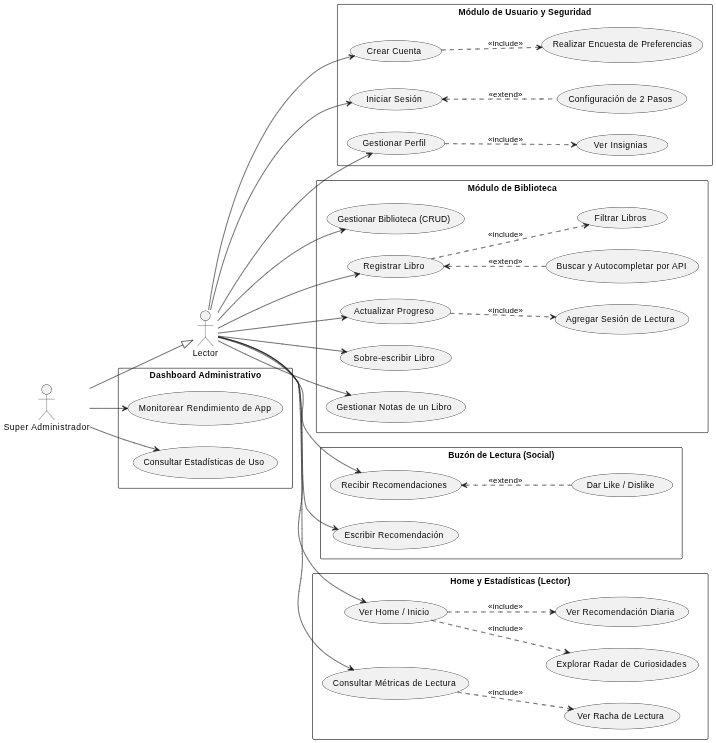
\includegraphics[width=1.0\textwidth]{./fotos/uc/image.png}
    \caption{Diagrama de casos de uso del sistema LecturaMétrica.}
    \label{fig:casos_de_uso}
\end{figure}

\subsection{Narrativas de casos de uso}
Las narrativas de casos de uso describen de manera concisa y estructurada las interacciones entre los actores y el sistema. A continuación, se presenta la especificación formal del caso de uso para el registro de sesiones, respetando estrictamente el formato y los parámetros definidos por el equipo de desarrollo:

\begin{table}[H]
\centering
\footnotesize
\begin{tabular}{|p{3.5cm}|p{10.5cm}|}
\hline
\textbf{Caso de Uso} & \textbf{UC-LIB-05 — Agregar Sesión de Lectura} \\ \hline
\textbf{Actor(es)} & Lector \\ \hline
\textbf{Precondiciones} & El libro está registrado en la biblioteca del lector. \\ \hline
\textbf{Flujo Normal} & 
\begin{minipage}{10cm}
\vspace{1mm}
\begin{enumerate}
    \item El usuario selecciona un libro y elige "Agregar sesión".
    \item El sistema solicita fecha, páginas leídas y tiempo invertido.
    \item El usuario completa los datos y confirma.
    \item El sistema registra la sesión y actualiza el progreso del libro (\textit{include} \textbf{UC-LIB-06}).
\end{enumerate}
\vspace{1mm}
\end{minipage} \\ \hline
\textbf{Flujo Alternativo} & 
\begin{minipage}{10cm}
\vspace{1mm}
\textbf{3a.} Las páginas ingresadas superan el total del libro: el sistema alerta y solicita corrección.
\vspace{1mm}
\end{minipage} \\ \hline
\textbf{Postcondiciones} & La sesión queda registrada y el progreso de lectura se actualiza. \\ \hline
\textbf{Include} & UC-LIB-06 Actualizar Progreso \\ \hline
\textbf{Extend} & — \\ \hline
\textbf{Prioridad} & Alta \\ \hline
\end{tabular}
\caption{Narrativa del caso de uso UC-LIB-05: Agregar Sesión de Lectura.}
\label{tab:uc_lib_05}
\end{table}

\begin{quote}
\textit{\textbf{Nota:} La tabla anterior (\ref{tab:uc_lib_05}) representa el formato estandarizado utilizado para la documentación de los requerimientos funcionales del proyecto. El catálogo completo con las demás narrativas elaboradas por el equipo se encuentra disponible en el \textbf{Anexo B: Especificación y Narrativas de Casos de Uso}.}
\end{quote}

\subsection{Modelo de datos preliminar (modelo ER)}
El modelo de datos preliminar, elaborado durante la fase de análisis del sistema, representa el diseño conceptual inicial de la información en \textbf{LecturaMétrica}. Este diagrama primigenio constaba de aproximadamente 13 entidades lógicas enfocadas en solventar los requerimientos funcionales básicos del dominio literario, abstrayéndose de los detalles de normalización y de la motorización relacional.

En su estructura original (modelo preliminar), el sistema agrupaba los elementos de la siguiente manera:
\begin{itemize}
    \item \textbf{Entidades Core:} \texttt{USUARIO}, \texttt{LIBRO}, \texttt{BIBLIOTECA}, \texttt{SESION\_LECTURA}, \texttt{RACHA} y \texttt{PERFIL}.
    \item \textbf{Catálogos y Relaciones Directas:} Tablas conceptuales como \texttt{GENERO}, \texttt{FORMATO}, \texttt{ESTADO\_LECTURA} e \texttt{INSIGNIA} que se relacionaban de manera directa, sin desglosar todavía las tablas intermedias de alta normalización.
    \item \textbf{Módulo Social y de Recomendaciones:} Entidades iniciales como \texttt{PREFERENCIA} y \texttt{BUZON\_RECOMENDACIONES} para el intercambio de cartas literarias.
\end{itemize}

\begin{figure}[H]
    \centering
    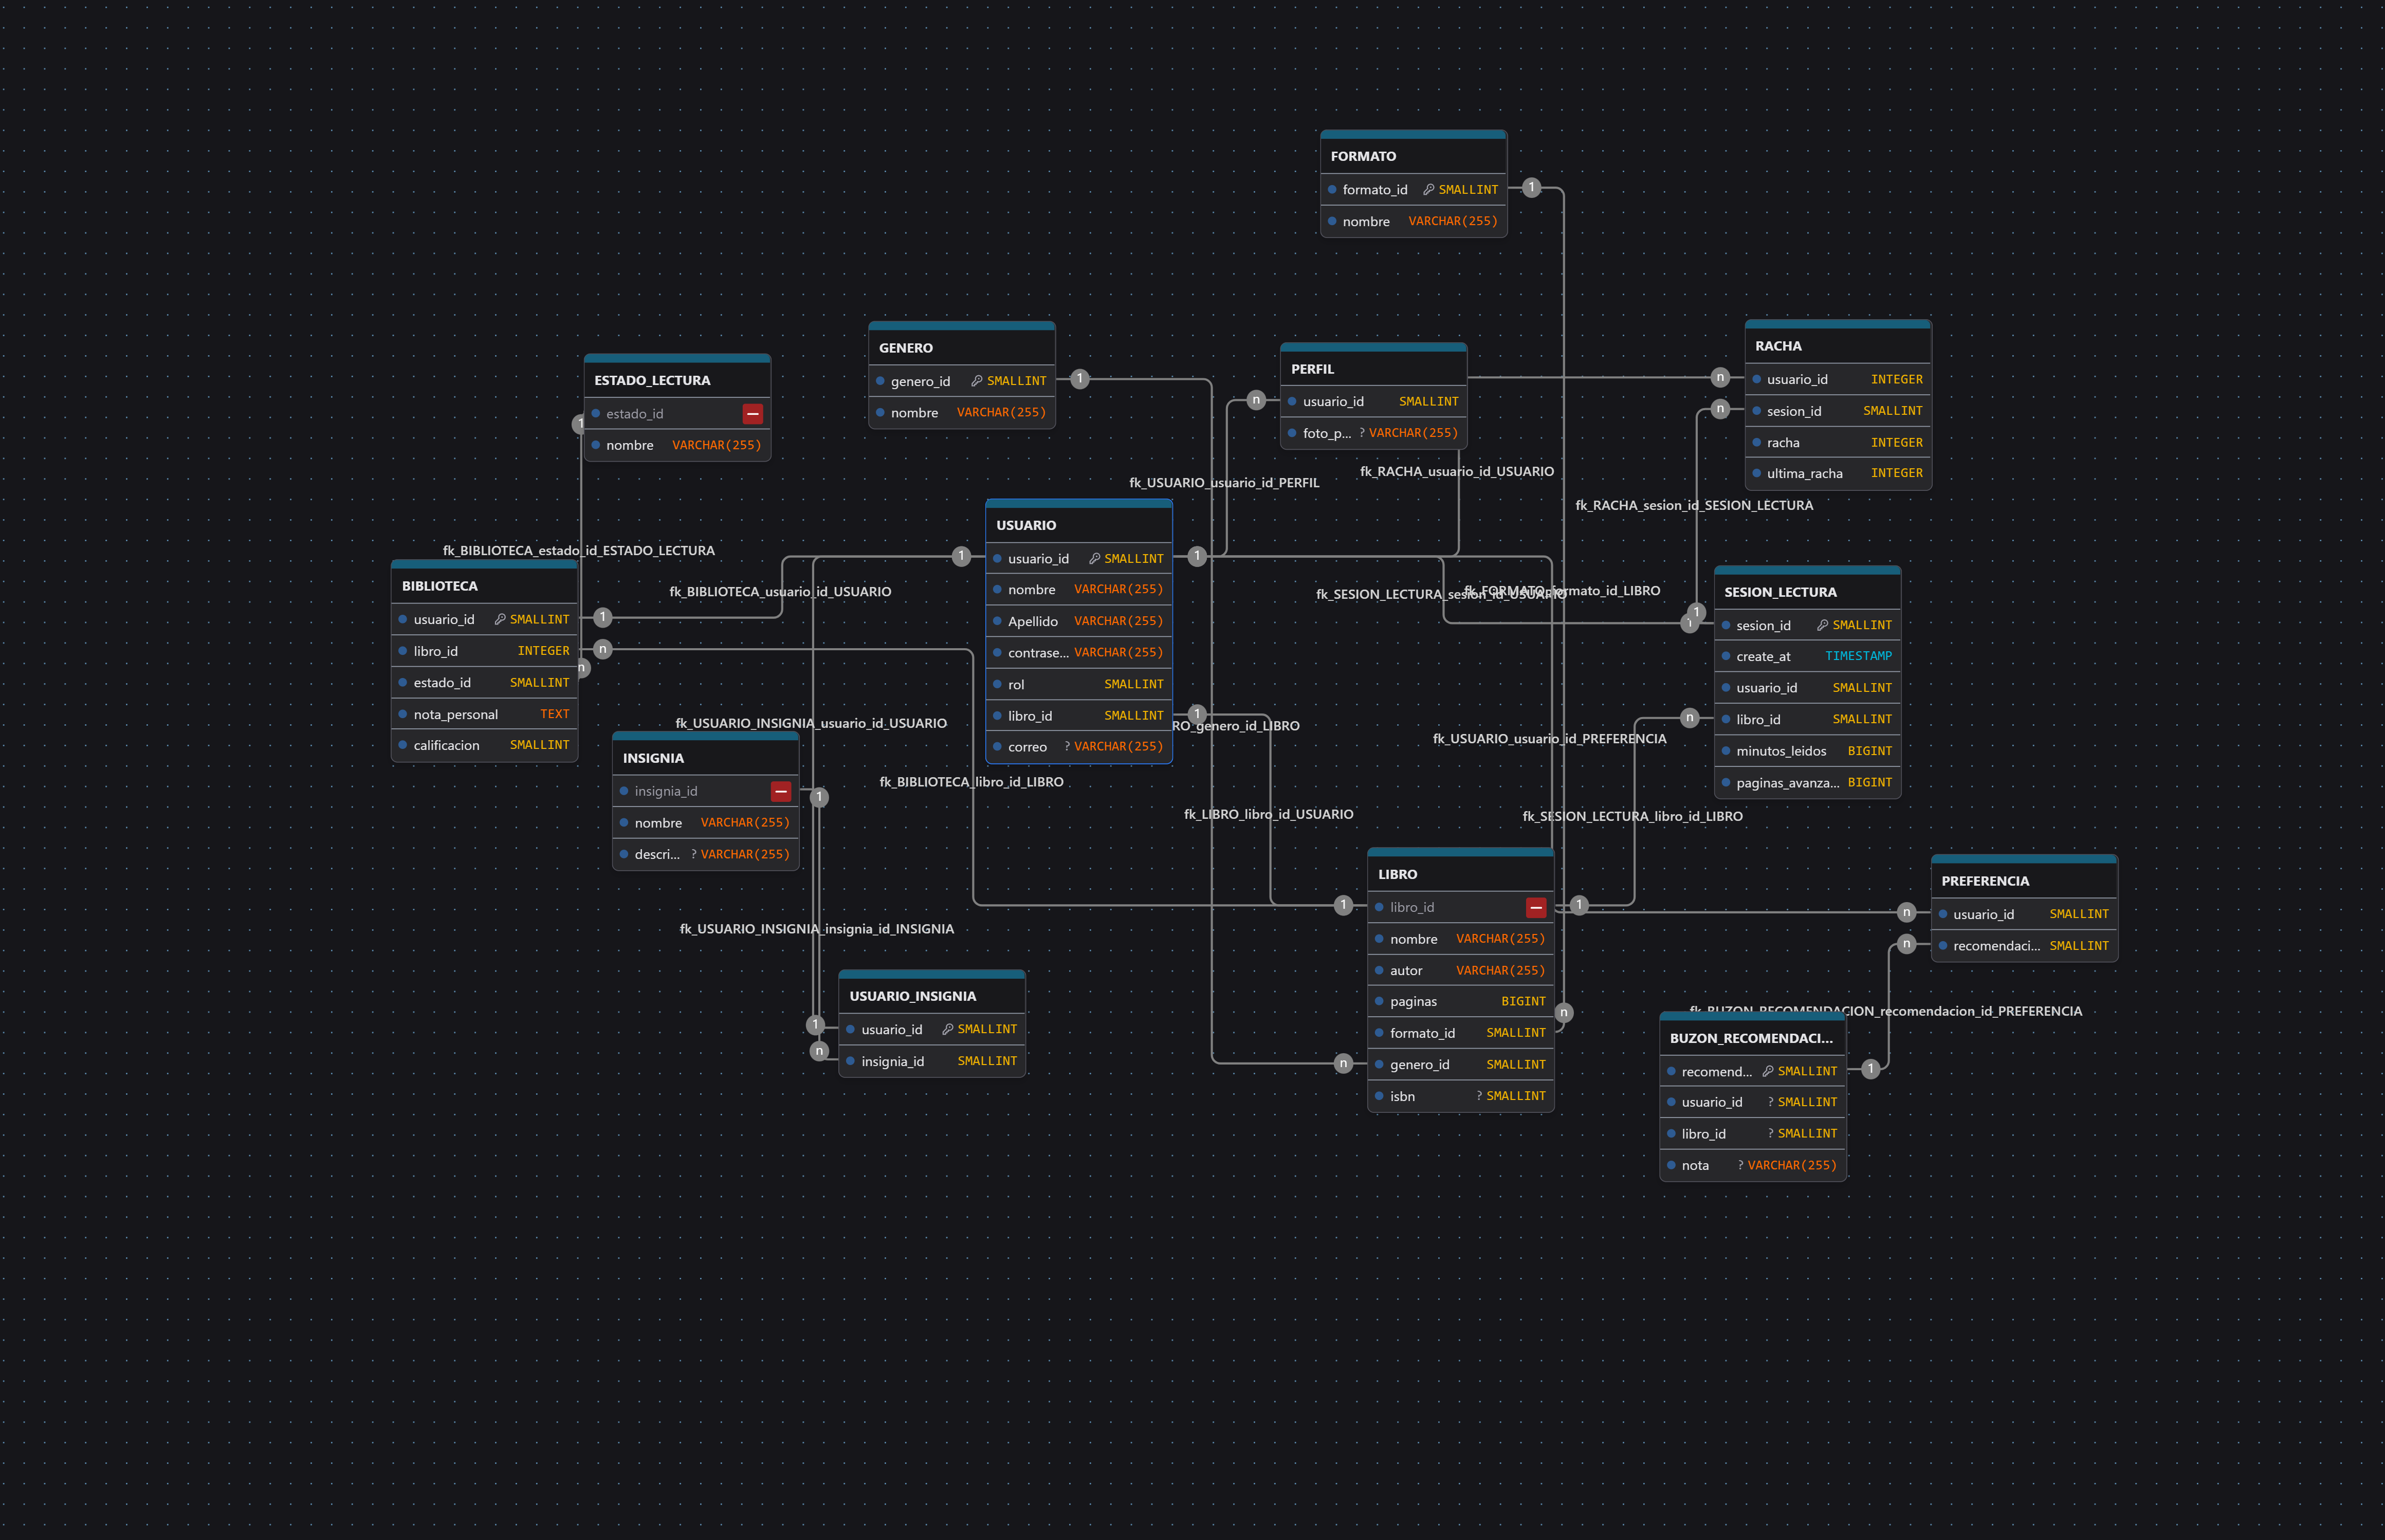
\includegraphics[width=1.0\textwidth]{./fotos/code/db.png}
    \caption{Modelo ER preliminar.}
    \label{fig:casos_de_uso}
\end{figure}


\subsection{Reglas del negocio}
Las reglas del negocio definen las condiciones lógicas, restricciones y políticas operativas que debe validar y hacer cumplir de manera estricta para asegurar la integridad de los datos y el correcto comportamiento del sistema:

\begin{itemize}
	\item \textbf{RN-01:} Toda obra agregada al catálogo debe asociarse obligatoriamente a un único formato principal (Libro, Manga, Manhwa, Cómic o Novela Gráfica).
	\item \textbf{RN-02:} La extensión total de una obra (expresada en páginas o capítulos) debe ser un número entero mayor a cero.
	\item \textbf{RN-03:} El progreso de lectura registrado por el usuario no puede exceder la extensión total definida para la obra ($0 \le \textit{Progreso Actual} \le \textit{Progreso Total}$).
	\item \textbf{RN-04:} Cuando el progreso actual alcance exactamente la extensión total de la obra (equivalente al 100\%), el estado de la lectura debe actualizarse automáticamente a \textit{Completado}.
	\item \textbf{RN-05:} Se considera que un día computa para la contabilización de la racha (\textit{streak}) si el usuario registra un incremento en el progreso de lectura mayor a cero dentro de dicho período.
	\item \textbf{RN-06:} Unicidad de credenciales: no pueden existir dos cuentas de usuario registradas con el mismo correo electrónico en la base de datos.
	\item \textbf{RN-07:} En caso de que un usuario ejecute la eliminación de su cuenta, el sistema debe efectuar un borrado en cascada de todas sus sesiones de lectura y notas asociadas, garantizando la privacidad de los datos y la integridad referencial.
	\item \textbf{RN-08:} Si una obra se clasifica bajo el estado \textit{Abandonado}, el sistema mantendrá y conservará el registro histórico del progreso alcanzado hasta ese momento.
\end{itemize}

\newpage

% ==============================================================================
% 9. DISEÑO DEL SISTEMA
% ==============================================================================
\section{Diseño del sistema}

\subsection{Arquitectura del sistema}
La arquitectura general de \textbf{LecturaMétrica} se fundamenta en un modelo clásico de \textbf{Arquitectura Cliente-Servidor}, evolucionado hacia un enfoque distribuido y desacoplado mediante servicios (API RESTful).

El proyecto se divide físicamente en repositorios independientes para las aplicaciones cliente y el servidor backend. Esta estructura evita el acoplamiento del código, permite un desarrollo modular y facilita la evolución autónoma de cada interfaz. El ecosistema opera bajo cuatro pilares fundamentales:

\begin{itemize}
    \item \textbf{Clientes de Usuario (Capa de Presentación):} Interfaces inteligentes y totalmente independientes del motor de base de datos, gestionan su propio enrutamiento visual y la experiencia de usuario:
    \begin{itemize}
        \item \textit{Aplicación Web Progresiva (PWA):} Aplicación para los lectores finales con adaptabilidad para dispositivos móviles y de escritorio.
        \item \textit{Dashboard de Administración:} Interfaz web simplificada para el personal de gestión.
    \end{itemize}
    
    \item \textbf{Servidor Central (API RESTful):} Núcleo de la lógica de negocio. Es un servicio backend independiente que recibe las peticiones HTTP de los clientes, procesa las reglas del sistema (cálculo de rachas de lectura, validaciones de seguridad y control de sesiones) y devuelve las respuestas en un formato estandarizado. Ningún cliente puede modificar datos sin pasar por la validación de este servidor.
    
    \item \textbf{Capa de Persistencia (Base de Datos):} El almacenamiento transaccional se encuentra aislado en un motor relacional (PostgreSQL). El servidor central es la única entidad autorizada para establecer conexión y ejecutar consultas o modificaciones sobre estas tablas, garantizando la seguridad y la integridad referencial de la información.
    
    \item \textbf{Sistemas y Servicios Externos:} El servidor central y los clientes se integran de manera controlada con herramientas de terceros, tales como la API de \textit{Open Library} para la obtención automática de metadatos literarios e ISBN, y \textit{Cloudinary} para el almacenamiento y optimización en la nube de recursos multimedia (portadas y avatares).
\end{itemize}

\subsubsection{Flujo de comunicación Cliente-Servidor}
La comunicación entre ambas capas se rige estrictamente por el ciclo de petición y respuesta (\textit{Request-Response}). Tanto la PWA como el Dashboard realizan peticiones asíncronas al servidor consumiendo puntos de acceso (\textit{endpoints}) protegidos. El intercambio de información se realiza mediante Objetos de Transferencia de Datos (\textit{DTOs}) estructurados en formato JSON a través del protocolo seguro HTTPS, asegurando que la interfaz visual y la lógica de almacenamiento trabajen en perfecta sincronía sin mezclar sus responsabilidades.

\subsection{Diseño de base de datos}

El almacenamiento transaccional de \textbf{LecturaMétrica} está implementado sobre el motor relacional \textbf{PostgreSQL}. El esquema fue diseñado bajo la tercera forma normal (3NF) para evitar la redundancia de datos y garantizar la integridad referencial a través de restricciones de llave foránea (\textit{Foreign Keys}).

\subsubsection{Decisiones estratégicas de diseño}
El modelado de la base de datos incorpora tres patrones arquitectónicos clave para optimizar la seguridad, el rendimiento y la trazabilidad del sistema:

\begin{itemize}
    \item \textbf{Estrategia híbrida de identificadores:} Las entidades transaccionales y de usuario (\texttt{users}, \texttt{books}, \texttt{user\_library}, \texttt{reading\_sessions}) utilizan identificadores únicos universales (\textbf{UUID}). Esto previene ataques de enumeración en la API y facilita la escalabilidad horizontal. Por otro lado, los catálogos y diccionarios (\texttt{authors}, \texttt{genders}, \texttt{formats}, \texttt{badges}) emplean enteros largos autoincrementables (\textbf{BIGINT}), optimizando el indexado y la velocidad de las consultas relacionales más frecuentes.
    \item \textbf{Trazabilidad y Borrado Suave (\textit{Soft Delete}):} Entidades principales como usuarios, libros, autores y estados integran banderas booleanas (\texttt{deleted}) y marcas de tiempo (\texttt{deleted\_at}). Esto permite desactivar registros en la lógica de negocio sin destruirlos físicamente, preservando la coherencia de las estadísticas e historiales de lectura.
    \item \textbf{Auditoría temporal:} La mayoría de las tablas incorporan atributos de control de tiempo (\texttt{created\_at}, \texttt{updated\_at}) para registrar el ciclo de vida de la información sin depender de bitácoras externas.
\end{itemize}

\subsubsection{Estructura relacional por dominios de negocio}
Para facilitar su comprensión y mantenimiento, el esquema de 22 tablas se agrupa en cinco dominios funcionales que reflejan directamente los módulos del backend:

\begin{table}[H]
\centering
\footnotesize
\begin{tabular}{|p{3.5cm}|p{2.3cm}|p{2cm}|p{5.5cm}|}
\hline
\textbf{Tabla} & \textbf{Llave Primaria} & \textbf{Tipo de Dato} & \textbf{Descripción y Responsabilidad} \\ \hline
\texttt{users} & \texttt{id} & \texttt{UUID} & Credenciales, metas anuales de lectura y relación con rol y fotografía. \\ \hline
\texttt{roles} & \texttt{id} & \texttt{UUID} & Catálogo de roles de acceso al sistema (Ej. Lector, Administrador). \\ \hline
\texttt{pictures} & \texttt{id} & \texttt{BIGINT} & Almacenamiento y URL de avatares sincronizados con Cloudinary. \\ \hline
\end{tabular}
\caption{Dominio 1: Gestión de Usuarios y Seguridad.}
\label{tab:db_users}
\end{table}

\begin{table}[H]
\centering
\footnotesize
\begin{tabular}{|p{3.5cm}|p{2.3cm}|p{2cm}|p{5.5cm}|}
\hline
\textbf{Tabla} & \textbf{Llave Primaria} & \textbf{Tipo de Dato} & \textbf{Descripción y Responsabilidad} \\ \hline
\texttt{books} & \texttt{id} & \texttt{UUID} & Catálogo central de obras literarias, código ISBN y URL de portada. \\ \hline
\texttt{authors} & \texttt{id} & \texttt{BIGINT} & Registro de autores literarios con soporte de borrado suave. \\ \hline
\texttt{genders} & \texttt{id} & \texttt{BIGINT} & Catálogo de géneros y clasificaciones literarias. \\ \hline
\texttt{formats} & \texttt{id} & \texttt{BIGINT} & Tipos de formato de lectura (Físico, Digital, Audiolibro). \\ \hline
\texttt{book\_authors} & \texttt{book\_id, author\_id} & \texttt{UUID / BIGINT} & Tabla intermedia para la relación N:M entre obras y autores. \\ \hline
\texttt{book\_genres} & \texttt{book\_id, gender\_id} & \texttt{UUID / BIGINT} & Tabla intermedia para la relación N:M entre obras y géneros. \\ \hline
\end{tabular}
\caption{Dominio 2: Catálogo Literario y Clasificación.}
\label{tab:db_books}
\end{table}

\begin{table}[H]
\centering
\footnotesize
\begin{tabular}{|p{3.5cm}|p{2.3cm}|p{2cm}|p{5.5cm}|}
\hline
\textbf{Tabla} & \textbf{Llave Primaria} & \textbf{Tipo de Dato} & \textbf{Descripción y Responsabilidad} \\ \hline
\texttt{user\_library} & \texttt{id} & \texttt{UUID} & Biblioteca personal del usuario, progreso actual y libro favorito. \\ \hline
\texttt{reading\_status} & \texttt{id} & \texttt{BIGINT} & Catálogo de estados de lectura (Por leer, Leyendo, Terminado). \\ \hline
\texttt{reading\_sessions}& \texttt{id} & \texttt{UUID} & Historial de lecturas con registro exacto de segundos, páginas y capítulos. \\ \hline
\texttt{library\_notes} & \texttt{id} & \texttt{BIGINT} & Notas y reflexiones guardadas por el usuario por página o capítulo. \\ \hline
\end{tabular}
\caption{Dominio 3: Biblioteca Personal, Sesiones y Notas.}
\label{tab:db_library}
\end{table}

\begin{table}[H]
\centering
\footnotesize
\begin{tabular}{|p{3.5cm}|p{2.3cm}|p{2cm}|p{5.5cm}|}
\hline
\textbf{Tabla} & \textbf{Llave Primaria} & \textbf{Tipo de Dato} & \textbf{Descripción y Responsabilidad} \\ \hline
\texttt{user\_streaks} & \texttt{id} & \texttt{UUID} & Control de racha actual, racha máxima y última fecha de actividad. \\ \hline
\texttt{badges} & \texttt{id} & \texttt{BIGINT} & Catálogo de insignias y recompensas visuales de la plataforma. \\ \hline
\texttt{user\_badges} & \texttt{id} & \texttt{BIGINT} & Registro de insignias y logros desbloqueados por cada usuario. \\ \hline
\texttt{curiosities} & \texttt{id} & \texttt{BIGINT} & Datos curiosos aleatorios para el radar de descubrimiento. \\ \hline
\end{tabular}
\caption{Dominio 4: Gamificación, Rachas y Descubrimiento.}
\label{tab:db_gamification}
\end{table}

\begin{table}[H]
\centering
\footnotesize
\begin{tabular}{|p{3.7cm}|p{2.1cm}|p{2cm}|p{5.5cm}|}
\hline
\textbf{Tabla} & \textbf{Llave Primaria} & \textbf{Tipo de Dato} & \textbf{Descripción y Responsabilidad} \\ \hline
\texttt{recommendations} & \texttt{id} & \texttt{UUID} & Perfil general de preferencias y configuración del lector. \\ \hline
\texttt{user\_pref\_formats} & \texttt{pref\_id, formats\_id} & \texttt{UUID / BIGINT} & Tabla intermedia que enlaza al usuario con sus formatos preferidos. \\ \hline
\texttt{user\_pref\_genres} & \texttt{pref\_id, genres\_id} & \texttt{UUID / BIGINT} & Tabla intermedia que enlaza al usuario con sus géneros preferidos. \\ \hline
\texttt{recommendation\_contents} & \texttt{id} & \texttt{BIGINT} & Contenido literario y mensajes para las recomendaciones creadas. \\ \hline
\texttt{letters} & \texttt{id} & \texttt{BIGINT} & Buzón de cartas para intercambio asíncrono y reclamo de lecturas. \\ \hline
\end{tabular}
\caption{Dominio 5: Recomendaciones y Buzón de Cartas.}
\label{tab:db_social}
\end{table}

\begin{figure}[H]
    \centering
    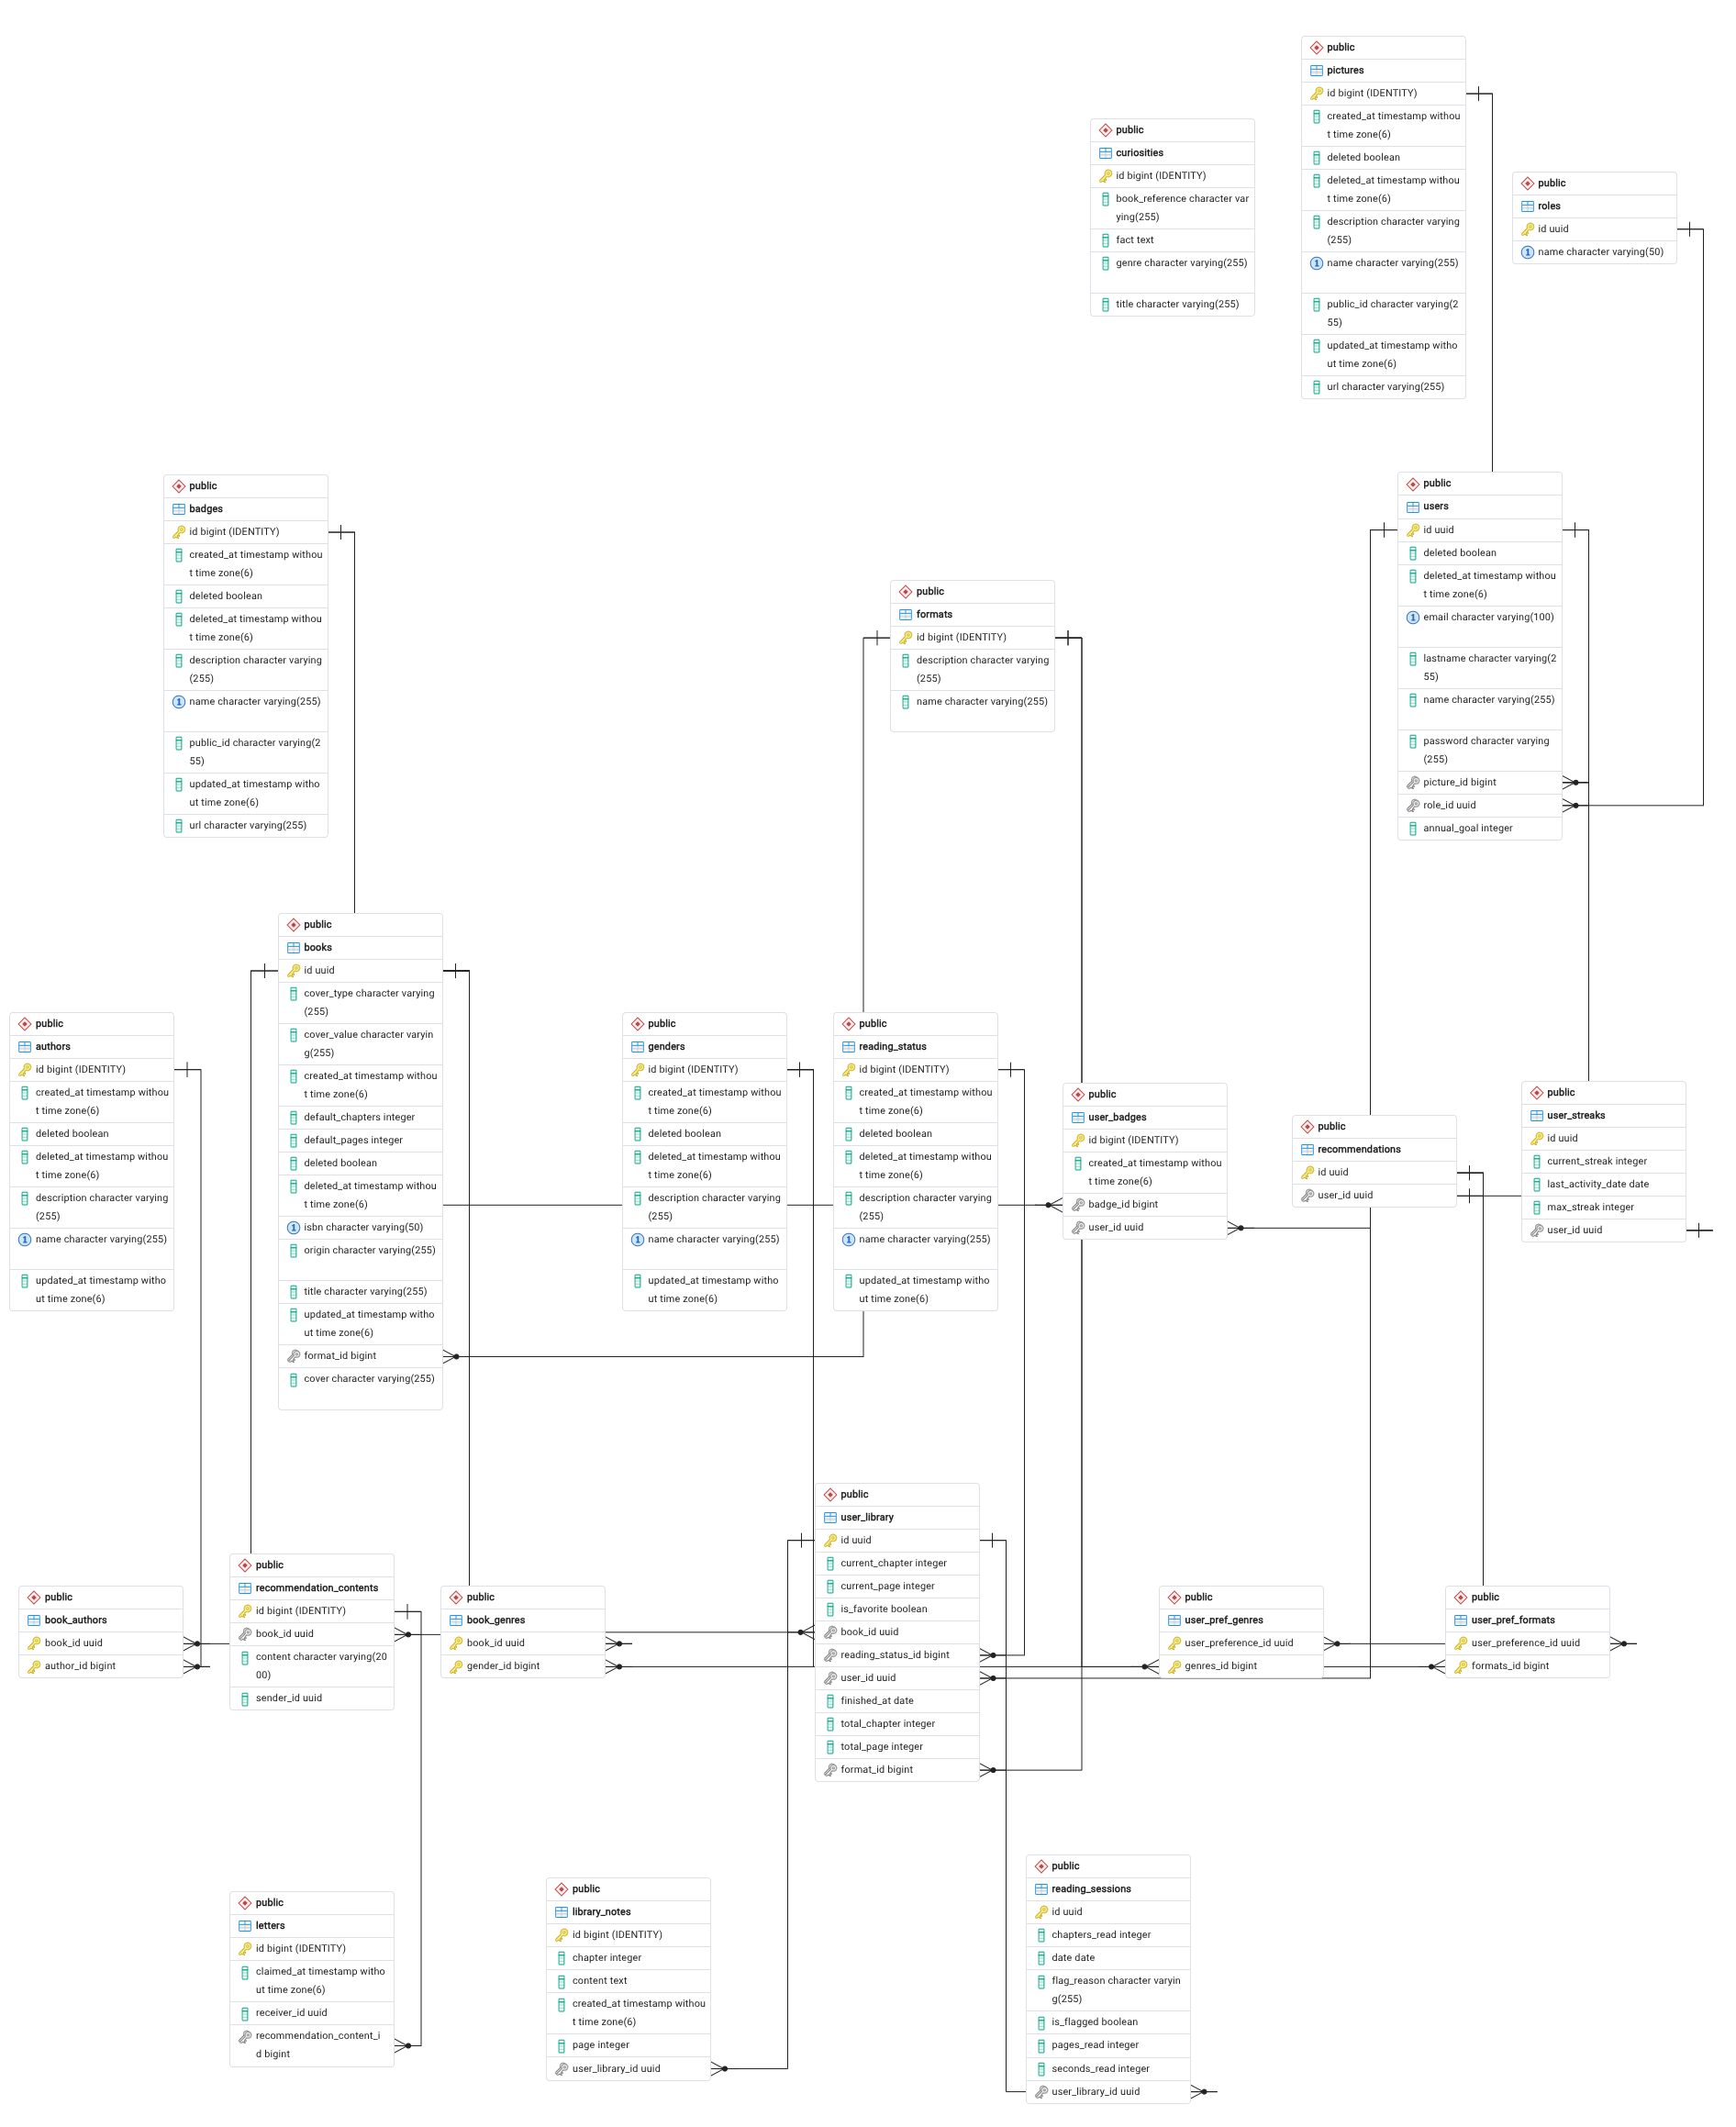
\includegraphics[width=0.9\textwidth]{./fotos/code/database.png}
    \caption{Diagrama Entidad-Relación de LecturaMétrica.}
    \label{fig:database}
\end{figure}

\subsubsection{Diccionario de datos y especificación técnica de columnas}
Para garantizar la integridad referencial y estandarizar el desarrollo entre el equipo de backend y base de datos, cada entidad del modelo relacional cuenta con una especificación estricta de tipos de datos, restricciones de nulidad y llaves de índice. 

A continuación, se presenta como muestra representativa la estructura técnica de la entidad central del negocio (\texttt{user\_library}), la cual gestiona la relación entre el lector y las obras de su catálogo personal:

\begin{table}[H]
    \centering
    \footnotesize
    \begin{tabular}{|l|l|c|p{6.5cm}|}
        \hline
        \textbf{Atributo} & \textbf{Tipo de Dato} & \textbf{Llave} & \textbf{Descripción y Restricción} \\ \hline
        \texttt{id} & \texttt{UUID} & PK & Identificador único e irrepetible del registro en la biblioteca. \\ \hline
        \texttt{user\_id} & \texttt{UUID} & FK & Referencia al propietario de la biblioteca \texttt{users(id)}. \\ \hline
        \texttt{book\_id} & \texttt{UUID} & FK & Referencia a la obra literaria \texttt{books(id)}. \\ \hline
        \texttt{format\_id} & \texttt{BIGINT} & FK & Referencia al formato de lectura \texttt{formats(id)}. \\ \hline
        \texttt{reading\_status\_id} & \texttt{BIGINT} & FK & Referencia al estado de lectura \texttt{reading\_status(id)}. \\ \hline
        \texttt{current\_page} & \texttt{INTEGER} & - & Página actual de avance ($0 \le \mathrm{valor} \le \mathrm{total\_page}$). \\ \hline
        \texttt{total\_page} & \texttt{INTEGER} & - & Total de páginas de la obra. \\ \hline
        \texttt{current\_chapter} & \texttt{INTEGER} & - & Capítulo actual de avance. \\ \hline
        \texttt{total\_chapter} & \texttt{INTEGER} & - & Total de capítulos de la obra. \\ \hline
        \texttt{is\_favorite} & \texttt{BOOLEAN} & - & Indicador booleano de obra favorita (por defecto \texttt{false}). \\ \hline
        \texttt{finished\_at} & \texttt{DATE} & - & Fecha en que el usuario completó la lectura (nulo si sigue leyendo). \\ \hline
    \end{tabular}
    \caption{Especificación técnica de columnas para la entidad \texttt{user\_library}.}
    \label{tab:sample_data_dictionary}
\end{table}

\vspace{0.2cm}

\begin{quote}
\textit{\textbf{Nota aclaratoria:} La tabla anterior (\ref{tab:sample_data_dictionary}) ilustra el estándar de modelado y tipado utilizado para la especificación física de la base de datos en PostgreSQL. Por cuestiones de legibilidad y para mantener la fluidez del presente documento técnico, el diccionario de datos exhaustivo con las especificaciones de las 22 tablas del sistema (incluyendo catálogos, tablas pivote $N:M$ y entidades de gamificación) se adjunta para su consulta integral en el \textbf{Anexo C: Diccionario de Datos del Sistema Relacional}.}
\end{quote}

\subsection{Diseño del backend}

El diseño del servidor de \textbf{LecturaMétrica} se fundamenta en los principios de la Arquitectura Limpia (\textit{Clean Architecture}). Esta decisión arquitectónica se tomó para desacoplar completamente la lógica central del negocio de las dependencias externas (como bases de datos, frameworks web y servicios de terceros), garantizando así un sistema escalable, mantenible y altamente testeable

El desarrollo se implementó en \textbf{Java 21} utilizando el ecosistema de \textbf{Spring Boot}, lo que facilita la inyección de dependencias y el mapeo objeto-relacional (ORM) a través de Spring Data JPA e Hibernate. 
Todo el código está organizado bajo un enfoque modular por características (\textit{Feature-driven structure}), donde cada dominio principal (como libros, usuarios, biblioteca, rachas y buzón) se encapsula de forma independiente.

\subsubsection{Estructura de capas por módulo}
Para asegurar la separación de responsabilidades, cada módulo dentro del sistema se subdivide estrictamente en tres capas lógicas.

\begin{enumerate}
    \item \textbf{Capa de Dominio:} Es el núcleo de la aplicación. Contiene las entidades (modelos de datos puros) y los eventos del dominio. Esta capa no tiene ninguna dependencia hacia Spring Boot u otras bibliotecas externas, asegurando que las reglas de negocio permanezcan puras.
    
    \item \textbf{Capa de Aplicación:} Contiene los casos de uso (\textit{Use Cases}) que orquestan la lógica del negocio. Ejemplos de esto son los servicios encargados de registrar nuevas obras, actualizar las rachas diarias de lectura o calcular el radar de preferencias del usuario.
    
    \item \textbf{Capa de Infraestructura (\textit{Infrastructure Layer}):} Es la capa más externa y se encarga de los detalles de implementación, se encuentran: 
    \begin{itemize}
        \item \textbf{Controladores REST (\textit{Routing/Controllers}):} Manejan las peticiones HTTP y exponen los \textit{endpoints} de comunicación .
        \item \textbf{Data Transfer Objects (DTOs) y Mapeadores:} Se aseguran de que las propiedades crudas de las peticiones no interactúen directamente con la capa de aplicación. Transforman los datos de entrada a modelos de dominio antes de ser procesados.
        \item \textbf{Repositorios:} Interfaces que gestionan la conexión directa con la base de datos PostgreSQL.
        \item \textbf{Clientes Externos (\textit{Clients}):} Adaptadores para comunicarse con APIs externas, utilizados principalmente para la ingesta de metadatos de los libros.
    \end{itemize}
\end{enumerate}

\subsubsection{Seguridad y Manejo Global de Excepciones}
La seguridad del backend se gestiona mediante filtros de autenticación y servicios de validación de tokens JWT para proteger los accesos, mientras que las contraseñas se almacenan de forma cifrada en la base de datos.

Adicionalmente, se configuró un manejador global de excepciones (\textit{Global Exception Handler}) a nivel de infraestructura para centralizar la captura de errores. Asegurando que siempre retorne un formato estructurado y predecible para el \textit{frontend}, en lugar de exponer las trazas de error internas del servidor.

\subsection{Diseño del frontend}

El diseño de la capa de presentación de \textbf{LecturaMétrica} se fundamenta en un modelo de componentes reactivos y tipado estático, utilizando \textbf{Next.js} junto con \textbf{TypeScript} y \textbf{Tailwind CSS}. Para mantener un bajo acoplamiento, optimizar el rendimiento y reforzar la seguridad, el desarrollo del cliente se dividió físicamente en dos repositorios independientes, separando por completo la experiencia de los lectores finales del panel de control administrativo.

Ambas interfaces utilizan el moderno sistema de Enrutamiento de Aplicaciones (\textit{App Router}) de Next.js, lo que permite organizar el código por dominios funcionales y aprovechar el renderizado optimizado para reducir los tiempos de carga en el navegador.

\subsubsection{Separación de aplicaciones por perfil de usuario}
La división en dos proyectos garantiza que cada interfaz cargue únicamente los recursos y lógica que necesita su perfil de usuario:

\begin{enumerate}
    \item \textbf{LecturaMétrica - Usuario (Aplicación Web Progresiva):}
    Es la interfaz principal orientada al consumidor. Está adaptada para funcionar de forma fluida tanto en dispositivos móviles como de escritorio (\textit{Responsive Design}). Su estructura de rutas en el directorio \texttt{app/} se organiza en tres flujos principales:
    \begin{itemize}
        \item \textbf{Autenticación y Registro \texttt{(auth)}:} Agrupa las vistas públicas de acceso, registro de cuentas, verificación de códigos de seguridad (\texttt{/verify-code}) y recuperación de contraseñas (\texttt{/forgot-password}).
        \item \textbf{Iniciación de Usuario \texttt{/onboarding}:} Un módulo dedicado a guiar a los nuevos usuarios en la configuración inicial de su perfil y preferencias de lectura.
        \item \textbf{Plataforma Principal \texttt{(app)}:} Contiene las vistas protegidas del lector, divididas en módulos claramente delimitados: gestión de catálogo personal (\texttt{/biblioteca}), temporizador asíncrono de sesiones en tiempo real (\texttt{/lectura}), visualización de gráficas y proyecciones (\texttt{/estadisticas}) y un sistema de mensajería para el intercambio de cartas literarias (\texttt{/buzon}).
    \end{itemize}
    
    \item \textbf{LecturaMétrica - Admin (Dashboard de Administración):}
    Es una plataforma web de control cerrado orientada al personal de gestión y soporte técnico. Al estar en un repositorio aislado, no compromete la ligereza del sistema de los usuarios finales. Su estructura se enfoca en la simplicidad operativa y la supervisión del ecosistema:
    \begin{itemize}
        \item \textbf{Acceso Seguro \texttt{(auth)}:} Módulo exclusivo para el inicio de sesión del personal administrativo.
        \item \textbf{Panel de Control \texttt{/dashboard}:} Subdividido en áreas estratégicas para el monitoreo general: métricas y proyecciones globales de la plataforma (\texttt{/resumen}), gestión de cuentas y roles (\texttt{/usuarios}) y un bitácora para el seguimiento del tráfico y comportamiento en el servidor (\texttt{/actividad}).
    \end{itemize}
\end{enumerate}

\subsubsection{Estructura interna y modularidad del código}
Para asegurar que el código sea mantenible y fácil de escalar por cualquier desarrollador, ambos repositorios siguen un patrón estándar de organización interna que separa la lógica visual de la comunicación externa:

\begin{itemize}
    \item \textbf{\texttt{app/}:} Contiene exclusivamente la lógica de enrutamiento, vistas de página (\texttt{page.tsx}) y plantillas de diseño generales (\texttt{layout.tsx}). Utiliza la convención de paréntesis, como \texttt{(app)} o \texttt{(auth)}, para crear "Grupos de Rutas" (\textit{Route Groups}); esto permite aplicar diseños de navegación específicos (por ejemplo, mostrar u ocultar barras laterales) sin alterar la dirección web en el navegador.
    
    \item \textbf{\texttt{components/}:} Almacena los bloques visuales reutilizables (botones, tarjetas de libros, tablas, barras de navegación y formularios de entrada). Estos componentes son agnósticos a las rutas, garantizando una consistencia visual en toda la interfaz.
    
    \item \textbf{\texttt{data/}:} Actúa como la capa de servicios del frontend. Aquí se centralizan todas las peticiones asíncronas hacia la API REST central (desarrollada en Spring Boot). Al aislar el consumo del servidor en este directorio, los componentes visuales se mantienen limpios y no necesitan conocer las URLs ni la lógica interna de los puntos de acceso HTTP.
    
    \item \textbf{\texttt{lib/} (en repositorio de Usuario):} Contiene funciones de utilidad general, validaciones de seguridad, formateadores de fechas y la lógica para el manejo del almacenamiento local de credenciales de sesión (tokens de autorización).
\end{itemize}

\subsubsection{Consumo de servicios y sincronización}
La comunicación entre ambas aplicaciones web y la API central se ejecuta en tiempo real mediante peticiones asíncronas. Cada vez que un usuario realiza una acción —como detener el cronómetro de lectura o filtrar un reporte administrativo—, el frontend procesa la información localmente, adjunta los tokens de seguridad pertinentes y transmite un Objeto de Transferencia de Datos (\textit{DTO}) en formato JSON hacia el backend. Esto permite actualizar la interfaz al instante, garantizando una experiencia interactiva sin la necesidad de recargar la página completa.

\newpage

% ==============================================================================
% 10. IMPLEMENTACIÓN
% ==============================================================================
\section{Implementación}

\subsection{Repositorios del proyecto y control de versiones}
El desarrollo del ecosistema \textbf{LecturaMétrica} se gestionó mediante el control de versiones distribuido Git y la plataforma de alojamiento GitHub. 

Para garantizar un bajo acoplamiento arquitectónico, mantener prácticas de Arquitectura Limpia y facilitar el ciclo de despliegue independiente de cada interfaz, el código fuente se encuentra versionado en tres repositorios oficiales:

\begin{table}[H]
\centering
\footnotesize
\begin{tabular}{|p{3.8cm}|p{6.2cm}|p{4.5cm}|}
\hline
\textbf{Módulo del Ecosistema} & \textbf{Responsabilidad y Tecnología} & \textbf{Enlace al Repositorio (GitHub)} \\ \hline
\textbf{Backend (API RESTful)} & Núcleo lógico del sistema, validación de reglas de negocio, cálculo de rachas y conexión a PostgreSQL. Desarrollado en Java y Spring Boot. & \url{https://github.com/SoftFairies/Backend.git} \\ \hline
\textbf{Frontend 1: Usuario (PWA)} & Aplicación Web Progresiva para lectores finales con cronómetro de lectura asíncrono y catálogo personal. Desarrollada en Next.js. & \url{https://github.com/SoftFairies/LecturaMetrica-Usuario.git} \\ \hline
\textbf{Frontend 2: Dashboard Admin} & Interfaz web cerrada (back-office) para la gestión de usuarios, monitoreo del sistema y administración de catálogo. Desarrollada en Next.js. & \url{https://github.com/SoftFairies/LecturaMetrica-Admin.git} \\ \hline
\end{tabular}
\caption{Repositorios oficiales y código fuente del sistema LecturaMétrica.}
\label{tab:repositorios_github}
\end{table}

\vspace{0.2cm}

La implementación del sistema comprende el desarrollo integral de la plataforma, dividiéndose en la construcción de la API RESTful (Backend) y la interfaz de usuario (Frontend).

\subsection{Estructura de carpetas}

\subsubsection{Frontend}
El desarrollo del cliente web se distribuye en dos repositorios independientes, utilizando el framework \textbf{Next.js} bajo el modelo de Enrutamiento de Aplicaciones (\path{App Router}) y \textbf{TypeScript} para el tipado estático. Esta organización permite desacoplar por completo la aplicación de los lectores de la plataforma administrativa.

\paragraph{1. Repositorio de Usuario (\textit{LecturaMétrica - PWA})}
Estructurado para ofrecer una experiencia interactiva en dispositivos móviles y de escritorio. El directorio \path{app/} hace uso de "Grupos de Rutas" mediante paréntesis (ej. \path{(app)} y \path{(auth)}) para aplicar diseños de navegación específicos y proteger vistas sin alterar la estructura de la URL web:

\begin{lstlisting}[language=bash, basicstyle=\ttfamily\footnotesize, breaklines=true, frame=single, showstringspaces=false, extendedchars=true]
LecturaMetrica-Usuario/
|-- app/
|   |-- (app)/             # Rutas protegidas de la plataforma principal
|   |   |-- biblioteca/    # Catálogo literario personal y filtros
|   |   |-- buzon/         # Sistema de mensajería para cartas literarias
|   |   |-- estadisticas/  # Visualización de métricas, proyecciones y rachas
|   |   `-- lectura/       # Cronómetro asíncrono y registro de sesiones
|   |-- (auth)/            # Flujos públicos de autenticación y seguridad
|   |   |-- forgot-password/
|   |   |-- login/
|   |   |-- register/
|   |   `-- verify-code/   # Verificación de códigos de seguridad 2FA/Email
|   `-- onboarding/        # Configuración inicial y preferencias del lector
|-- components/            # Componentes visuales reutilizables
|-- data/                  # Consumo de servicios y comunicación con la API|
`-- lib/                   # Utilidades generales, validaciones y manejo de sesión
\end{lstlisting}

\paragraph{2. Repositorio de Administración (\textit{LecturaMétrica - Dashboard})}
Estructurado como un panel de control back-office optimizado para la carga e inspección de datos masivos. Se aísla de las dependencias de la PWA para garantizar ligereza y seguridad operativa:

\begin{lstlisting}[language=bash, basicstyle=\ttfamily\footnotesize, breaklines=true, frame=single, showstringspaces=false, extendedchars=true]
LecturaMetrica-Admin/
|-- app/
|   |-- (auth)/            # Acceso restringido para el personal administrativo
|   |   `-- login/
|   `-- dashboard/         # Panel de control y supervisión del ecosistema
|       |-- actividad/     # Bitácora de tráfico y monitoreo de eventos
|       |-- resumen/       # Métricas generales y proyecciones de la plataforma
|       `-- usuarios/      # Gestión de roles, permisos y cuentas
|-- components/            # Tablas de datos con paginación, filtros y modales
`-- data/                  # Peticiones HTTP y servicios de integración con Spring Boot
\end{lstlisting}

\paragraph{Separación de responsabilidades en el Frontend}
Para mantener un código limpio y modular, ambos repositorios comparten la misma lógica de organización arquitectónica en sus directorios raíz:
\begin{itemize}
    \item \textbf{\path{app/}:} Contiene únicamente las páginas visuales (\path{page.tsx}), plantillas maestras (\path{layout.tsx}) y la configuración del enrutador. No almacena lógica de peticiones HTTP ni utilidades complejas.
    \item \textbf{\path{components/}:} Aloja los bloques constructivos de la interfaz. Al ser modulares y agnósticos al enrutamiento, garantizan que un cambio visual en un botón o tabla se refleje de manera uniforme en todo el sistema.
    \item \textbf{\path{data/}:} Centraliza la capa de servicios. Actúa como el único punto de contacto entre la interfaz visual y el Backend en Spring Boot, aislando las llamadas asíncronas (\path{fetch}) y el manejo de cabeceras de autorización de los componentes visuales.
\end{itemize}

\subsubsection{Backend (API REST)}
El backend está desarrollado en Java con Spring Boot, estructurado bajo una arquitectura modular orientada al dominio. Cada módulo agrupa las capas de aplicación (casos de uso), dominio (modelos) e infraestructura (controladores, repositorios y clientes externos).

\begin{lstlisting}[language=bash, basicstyle=\ttfamily\footnotesize, breaklines=true, frame=single, showstringspaces=false, extendedchars=true]
src/main/java/com/fairies/api/proyecto/
|-- Application.java
|-- common
|   |-- application
|   |   `-- security      # Interfaces y contratos.
|   |-- domain
|   |   `-- service       # Contratos de servicios de almacenamiento
|   `-- infrastructure
|       |-- config        # Configuraciones generales y OpenAPI/Swagger
|       |-- rest          # Manejo global de excepciones y DTOs comunes
|       |-- security      # Filtros JWT y cifrado BCrypt
|       `-- service       # Implementación de Cloudinary
`-- modules/              # Módulos del sistema
   |-- auth/              # Autenticación y registro (Login/Sign-up)
   |-- author/            # Gestión de autores
   |-- badge              # Gestión de insignias
   |-- book               # Catálogo de libros
   |   `-- infrastructure
   |       `-- client     # Consumo de API externa (OpenLibrary)
   |-- Curiosityradar     # Recomendador aleatorio de curiosidades
   |-- format             # Gestión de formatos de lectura
   |-- gamification       # Asignación de insignias al usuario
   |-- gender             # Gestión géneros literarios
   |-- library            # Biblioteca personal y notas de lectura
   |-- mailbox            # Intercambio de cartas asincronas
   |-- picture            # Gestión de avatares
   |-- readingsession     # Sesiones, páginas y tiempo de lectura
   |-- readingStatus      # Gestión de estados de lectura 
   |-- recommendation     # Preferencias de lectura
   |-- reports            # Proyecciones y métricas del dashboard
   |-- streak             # Control de racha continua y eventos
   `-- user               # Gestión de usuarios y roles
\end{lstlisting}

Cada uno de los módulos de negocio mantiene una separación estricta de responsabilidades.
\begin{itemize}\sloppy
    \item \textbf{domain/}: Contiene los modelos de entidad (ej. \path{Book}, \path{UserLibrary}) y eventos de dominio (\path{StreakTriggerEvent}).
    \item \textbf{application/}: Aloja los casos de uso (\textit{Use Cases}) con la lógica de negocio pura (ej. \path{AddReadingSessionUseCase}, \path{AwardBadgeUseCase}).
    \item \textbf{infrastructure/}: Implementa la persistencia (\path{JPARepository}), controladores REST (\path{Routing}), mappers (\path{MapStruct}) y DTOs de entrada/salida.
\end{itemize}



\subsection{Fragmentos de código clave}

\subsubsection{Carga Asíncrona y Resiliente de Catálogos (Frontend - \texttt{BibliotecaPage})}
Para garantizar que la interfaz en Next.js no se bloquee ni falle en caso de latencia o errores de red en el servidor, el componente de la biblioteca implementa un patrón de carga paralela con degradación elegante (\textit{Graceful Degradation}). 

Mediante la función \texttt{loadCatalogs}, se ejecutan cuatro peticiones HTTP en paralelo utilizando \texttt{Promise.all} para consultar los géneros, formatos, estados de lectura y autores desde la API REST. Cada llamada incorpora su propio bloque de captura de excepciones (\texttt{.catch()}) con arreglos vacíos o constantes de respaldo (\texttt{FALLBACK\_STATUSES}), asegurando que el formulario de creación de libros siga funcionando para el usuario incluso si alguno de los catálogos secundarios del backend no se encuentra disponible:

\begin{lstlisting}[language=Java, basicstyle=\ttfamily\footnotesize, breaklines=true, frame=single, showstringspaces=false]
useEffect(() => {
  const loadCatalogs = async () => {
    try {
      // Ejecución paralela de 4 peticiones a la API con sus propios respaldos de error
      const results = await Promise.all([
        api.genders.getAll({ page: 0, size: 50 }).catch(() => ({ content: [] as CatalogItem[] })),
        api.formats.getAll({ page: 0, size: 50 }).catch(() => ({ content: [] as CatalogItem[] })),
        api.readingStatus
          .getAll({ page: 0, size: 50 })
          .catch(() => ({ content: FALLBACK_STATUSES })),
        api.authors.getAll({ page: 0, size: 300 }).catch(() => ({ content: [] as CatalogItem[] })),
      ]);

      const genrePage = results[0];
      const formatPage = results[1];
      const statusPage = results[2];
      const authorPage = results[3];

      // Sincronización con el estado local de React
      setGenres(genrePage.content || []);
      setFormats(formatPage.content || []);
      setStatuses(
        statusPage.content && statusPage.content.length ? statusPage.content : FALLBACK_STATUSES,
      );
      setAuthors(authorPage.content || []);

      // Autoselección inteligente del primer formato disponible
      setFormatId((current) =>
        current === "" && formatPage.content && formatPage.content[0]
          ? formatPage.content[0].id
          : current,
      );
    } catch {
      // Restablecimiento a valores seguros si falla la promesa global
      setGenres([]);
      setFormats([]);
      setStatuses(FALLBACK_STATUSES);
      setAuthors([]);
    }
  };

  void loadCatalogs();
}, []);
\end{lstlisting}

\subsubsection{Inicialización Segura y Tolerancia a Fallos (Frontend - \texttt{LecturaPage})}
La vista de registro de sesiones de lectura requiere sincronizar múltiples fuentes de datos al montarse en el navegador. Para evitar que problemas de red en servicios secundarios bloqueen la operativa principal del usuario, el componente implementa un patrón de aislamiento de fallos dentro de su ciclo de vida reactivo.

Como se observa en el siguiente fragmento, la petición para obtener las rachas del usuario (\texttt{api.streaks.getMine}) se encapsula en un bloque de captura independiente dentro del flujo principal de carga de la biblioteca (\texttt{api.library.getAll}). Adicionalmente, se integra una bandera de control (\texttt{active}) para prevenir fugas de memoria y errores por condiciones de carrera si el usuario abandona la vista antes de que finalicen las promesas asíncronas:

\begin{lstlisting}[language=Java, basicstyle=\ttfamily\footnotesize, breaklines=true, frame=single, showstringspaces=false]
useEffect(() => {
  let active = true;

  const load = async () => {
    try {
      setLoadingBook(true);

      // Carga principal de la biblioteca
      const libraryPage = await api.library.getAll({ page: 0, size: 100 });
      if (!active) return;

      // Aislamiento de fallos: La racha se consulta en su propio bloque try-catch
      // Si el servicio de rachas falla, no interrumpe la carga del libro
      try {
        const streak = await api.streaks.getMine();
        if (active) {
          setCurrentStreak(Number(streak.currentStreak ?? 0));
          setMaxStreak(Number(streak.maxStreak ?? 0));
        }
      } catch {
        if (active) {
          setCurrentStreak(0);
          setMaxStreak(0);
        }
      }

      // Normalización defensiva de la respuesta de la API
      const safeLibs: LibraryItem[] = Array.isArray(libraryPage)
        ? libraryPage
        : libraryPage.content || [];

      setLibraryItems(safeLibs);

      if (safeLibs.length === 0) {
        clearReadingSelection();
        return;
      }

      // Recuperación inteligente del último libro seleccionado en la sesión local
      const storedSelectedId =
        typeof window !== "undefined"
          ? window.localStorage.getItem(SELECTED_READING_BOOK_KEY)
          : null;

      const selectedBook =
        safeLibs.find((item) => item.id === storedSelectedId) ||
        safeLibs.find((item) => item.readingStatusName?.toLowerCase() === "leyendo") ||
        safeLibs[0];

      await applyLibraryItem(selectedBook);
    } catch (error) {
      console.error("Error cargando libro de lectura:", error);
      await Swal.fire({
        icon: "error",
        title: "Error",
        text: "No se pudo cargar tu biblioteca para iniciar la sesión.",
      });
    } finally {
      if (active) setLoadingBook(false);
    }
  };

  void load();

  // Limpieza al desmontar el componente para prevenir fugas de memoria
  return () => {
    active = false;
  };
}, []);
\end{lstlisting}

\subsubsection{Consumo de API Externa (\texttt{OpenLibraryClient})}
El cliente gestiona la petición HTTP a la API de Open Library y procesa la respuesta mediante registros internos para extraer los metadatos esenciales de forma eficiente:

\begin{lstlisting}[language=Java, basicstyle=\ttfamily\footnotesize, breaklines=true, frame=single]
@Override
public List<CreateBookRequest> searchExternalBooks(String query) {
    String url = "https://openlibrary.org/search.json?q=" + query +
            "&limit=5&fields=title,author_name,isbn,subject,cover_i";
    List<CreateBookRequest> results = new ArrayList<>();
    
    try {
        var response = restTemplate.getForObject(url, OpenLibraryResponse.class);
        if (response != null && response.docs() != null) {
            for (Doc info : response.docs()) {
                String isbn = (info.isbn() != null && !info.isbn().isEmpty())
                        ? info.isbn().get(0) : "EXT-" + UUID.randomUUID().toString().substring(0, 8);
                
                String cover = info.cover_i() != null ?
                        "https://covers.openlibrary.org/b/id/" + info.cover_i() + "-M.jpg" : null;

                results.add(new CreateBookRequest(isbn, info.title(), null, null, cover));
            }
        }
    } catch (Exception e) {
        System.err.println("Error al consumir OpenLibrary API: " + e.getMessage());
    }
    return results;
}
\end{lstlisting}

\subsubsection{Control y Actualización de Rachas (\texttt{UpdateUserStreakUseCase})}
Este algoritmo compara la fecha actual con la última actividad registrada para incrementar o reiniciar de forma atómica la racha de lectura del usuario:

\begin{lstlisting}[language=Java, basicstyle=\ttfamily\footnotesize, breaklines=true, frame=single]
@Transactional(propagation = Propagation.REQUIRES_NEW)
public void execute(UUID userId) {
    LocalDate today = dateProvider.getToday();
    UserStreak streak = userStreakRepository.findByUserId(userId)
            .orElseGet(() -> createInitialStreak(userId));

    if (streak.getLastActivityDate() == null) {
        streak.setCurrentStreak(1);
        streak.setMaxStreak(1);
    } else if (streak.getLastActivityDate().equals(today)) {
        return; // Ya registró actividad hoy
    } else if (streak.getLastActivityDate().equals(today.minusDays(1))) {
        streak.setCurrentStreak(streak.getCurrentStreak() + 1);
        if (streak.getCurrentStreak() > streak.getMaxStreak()) {
            streak.setMaxStreak(streak.getCurrentStreak());
        }
    } else {
        streak.setCurrentStreak(1); // Racha rota
    }

    streak.setLastActivityDate(today);
    userStreakRepository.save(streak);
}
\end{lstlisting}

\subsubsection{Lógica de Negocio y Progreso (\texttt{AddReadingSessionUseCase})}
Este componente procesa el avance de páginas y capítulos, evalúa si el libro ha sido completado y dispara de forma asíncrona los eventos para actualizar la racha y otorgar insignias:

\begin{lstlisting}[language=Java, basicstyle=\ttfamily\footnotesize, breaklines=true, frame=single]
@Transactional
public ReadingSession execute(UUID userId, UUID libraryId, ReadingSessionRequest request) {
    UserLibrary userLibrary = libraryRepository.findById(libraryId)
            .filter(lib -> lib.getUser().getId().equals(userId))
            .orElseThrow(() -> new ResourceNotFoundException("Library not found."));

    userLibrary.setCurrentPage(userLibrary.getCurrentPage() + request.pagesRead());
    
    if (userLibrary.getCurrentPage() >= userLibrary.getTotalPage()) {
        var completedStatus = readingStatusRepository.findById(3L).orElseThrow();
        userLibrary.setReadingStatus(completedStatus);
        userLibrary.setFinishedAt(LocalDate.now());
    }

    ReadingSession session = sessionRepository.save(ReadingSession.builder()
            .userLibrary(userLibrary)
            .date(request.date() != null ? request.date() : LocalDate.now())
            .secondsRead(request.secondsRead())
            .pagesRead(request.pagesRead())
            .build());

    eventPublisher.publishEvent(new StreakTriggerEvent(userId));
    return session;
}
\end{lstlisting}



\subsection{Evidencia visual}

\subsubsection{Consumo de Servicios e Interfaz (Frontend)}

\begin{figure}[H]
    \centering
    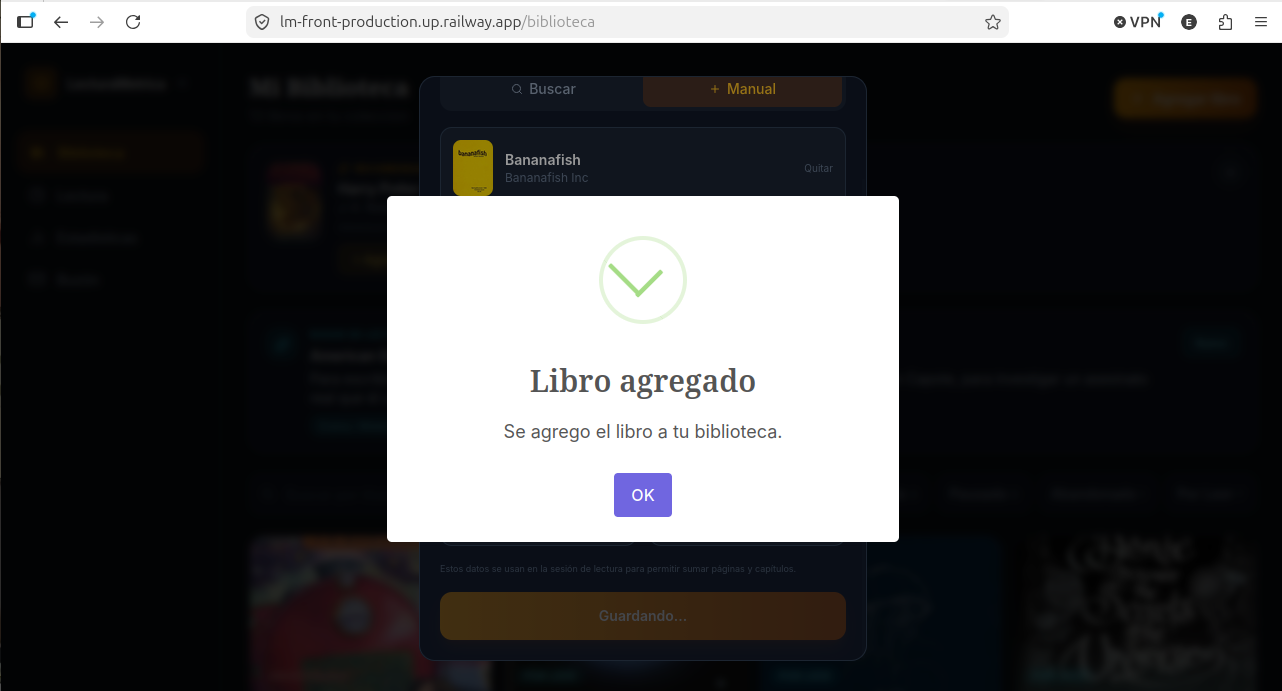
\includegraphics[width=0.9\textwidth]{./fotos/vistas/usuario/AgregarLibro(Exito).png}
    \caption{Agregar un libro a la biblioteca personal.}
    \label{fig:vista_usuario_agregar_libro}
\end{figure}

\begin{figure}[H]
    \centering
    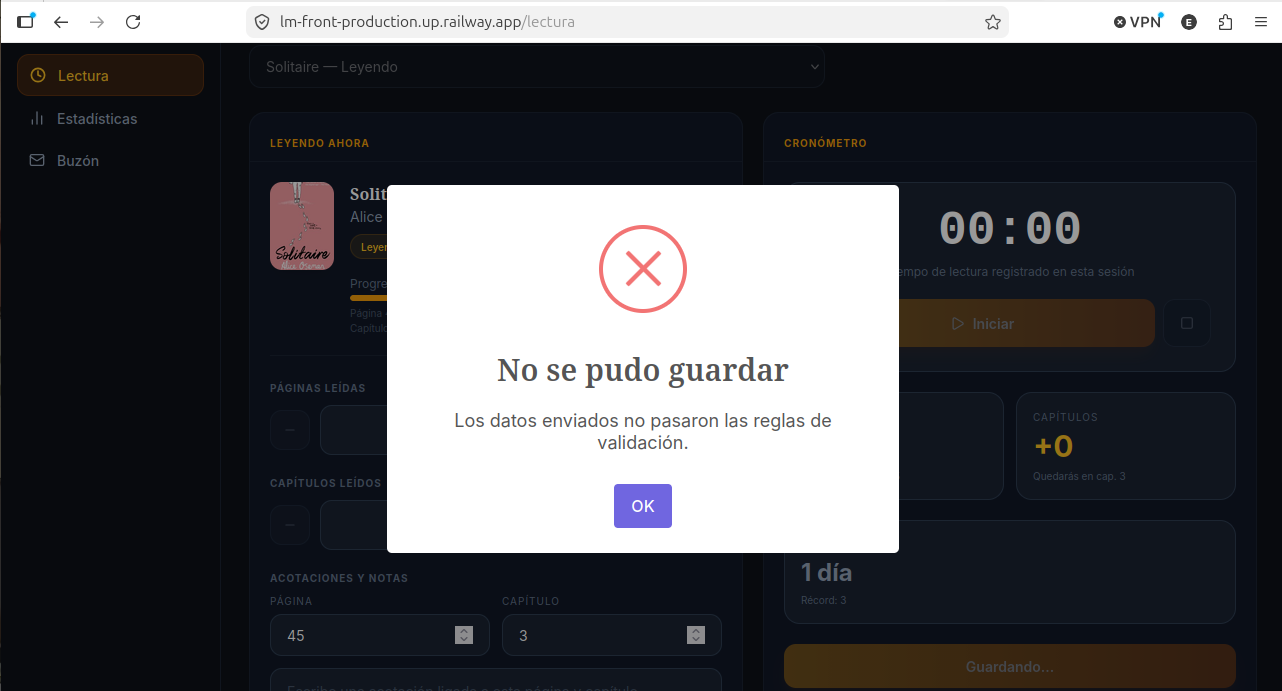
\includegraphics[width=0.9\textwidth]{./fotos/vistas/usuario/SesionLectura(Fallido).png}
    \caption{Agregar una sesión de lectura fallida para actualizar el progreso de un libro.}
    \label{fig:vista_usuario_agregar_sesion_fallida}
\end{figure}

\begin{figure}[H]
    \centering
    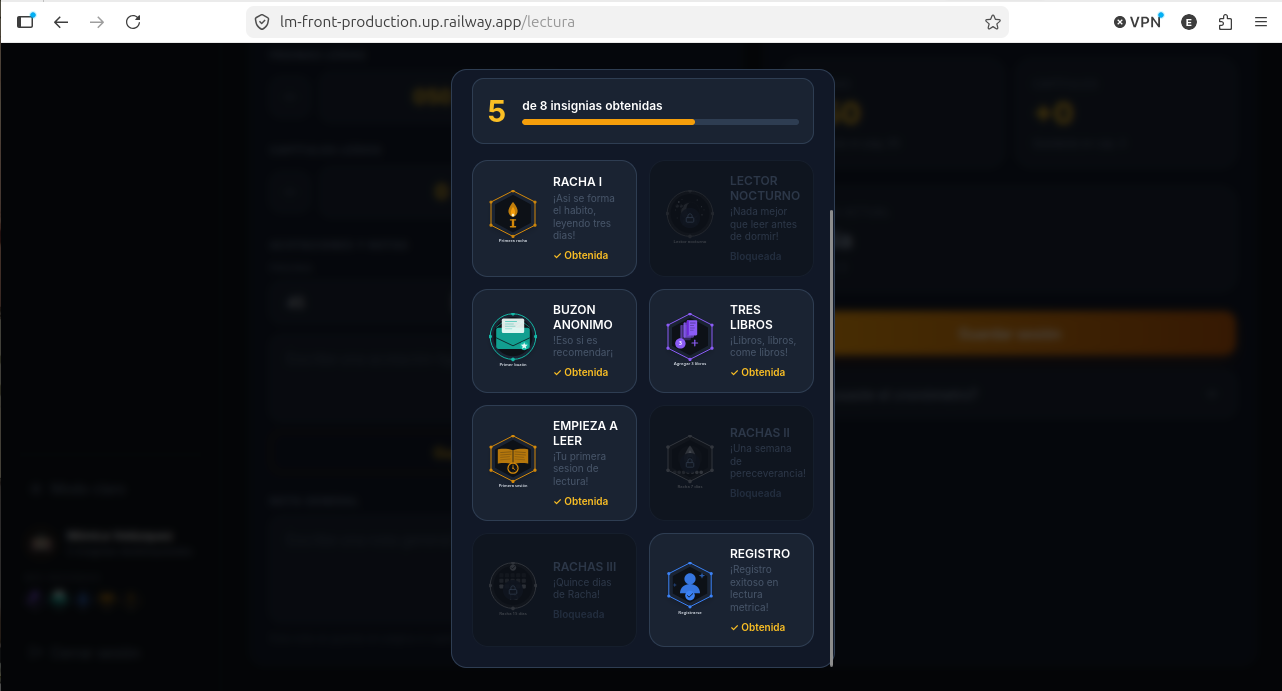
\includegraphics[width=0.9\textwidth]{./fotos/vistas/usuario/PerfilInsignias.png}
    \caption{Gamificación por medio de insignias.}
    \label{fig:vista_usuario_insignias}
\end{figure}

\subsubsection{Pruebas y Documentación de API (Backend)}
La correcta funcionalidad de los endpoints del backend se validó a través de herramientas de prueba de peticiones HTTP y la interfaz interactiva de documentación OpenAPI / Swagger UI:

\begin{figure}[H]
    \centering
    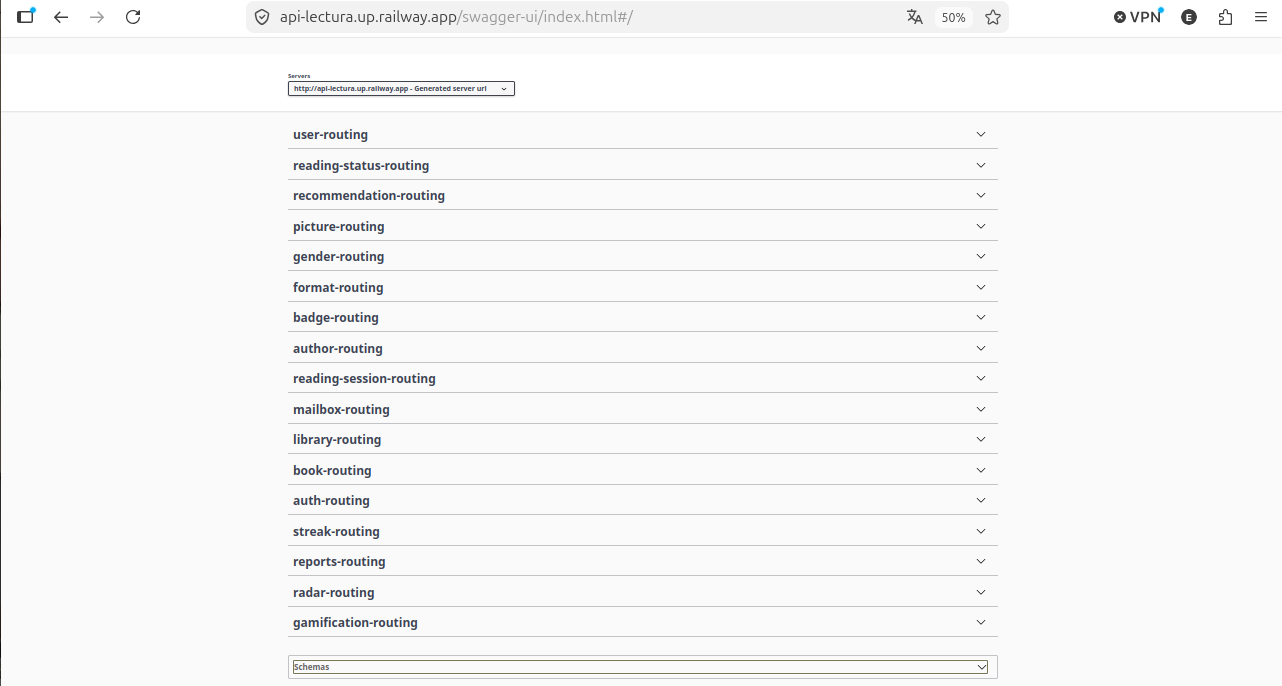
\includegraphics[width=0.9\textwidth]{./fotos/swagger/swagger-docs.png}
    \caption{Documentación de endpoints del backend en Swagger UI.}
    \label{fig:swagger_docs}
\end{figure}

\begin{figure}[H]
    \centering
    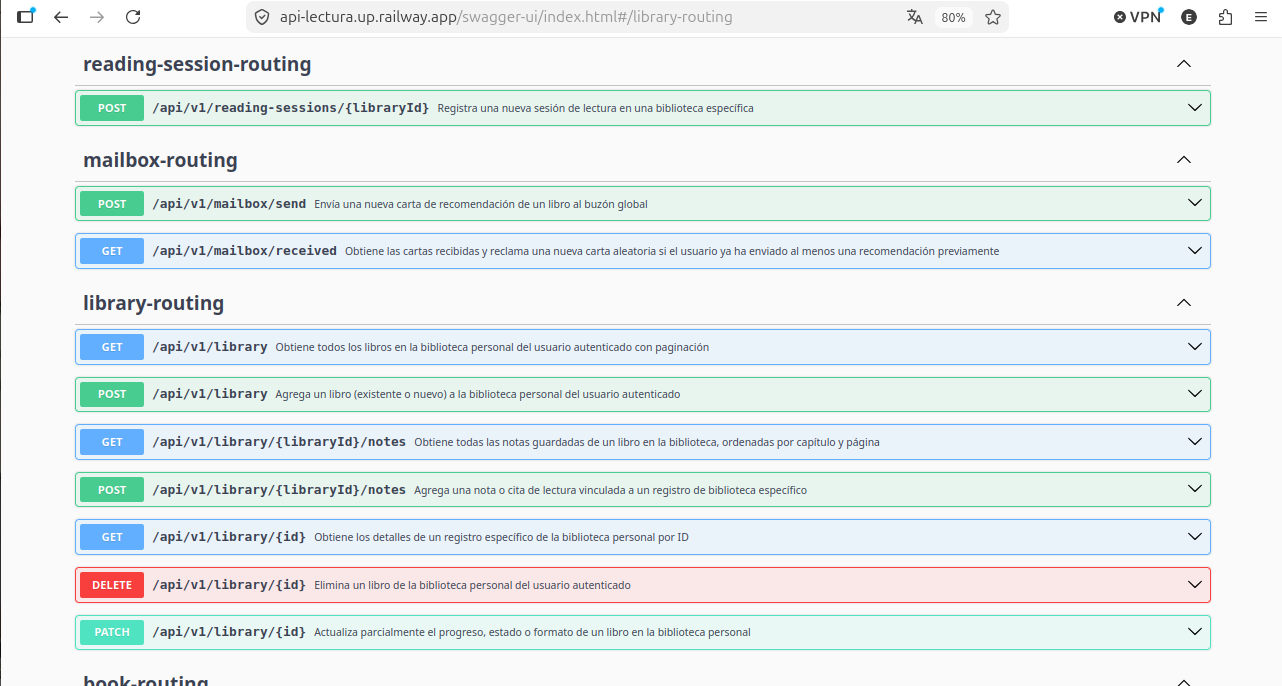
\includegraphics[width=0.9\textwidth]{./fotos/swagger/uno.png}
    \caption{Vista de documentación de 4 recursos del backend en Swagger UI.}
    \label{fig:swagger_docs_dos}
\end{figure}

% ==============================================================================
% 11. PRUEBAS
% ==============================================================================
\section{Pruebas}

\subsection{Casos de prueba}
En esta sección se describen los escenarios de prueba ejecutados sobre el sistema para validar el funcionamiento de los módulos principales, el cumplimiento de las reglas del negocio y el manejo de respuestas del servidor:

\begin{table}[h]
	\centering
	\small
	\caption{Matriz de ejecución de casos de prueba del sistema}
	\label{tab:casos_prueba}
	\begin{tabular}{p{1.2cm}p{2.3cm}p{3.2cm}p{3.5cm}p{3.5cm}}
		\toprule
		\textbf{ID} & \textbf{Módulo} & \textbf{Caso de Prueba} & \textbf{Acción / Entrada} & \textbf{Resultado Esperado} \\
		\midrule
		\textbf{CP-01} & Autenticación & Inicio de sesión exitoso de un Administrador. & Ingresar correo y contraseña válidos en \texttt{app/(auth)} y enviar el formulario. & El \textit{backend} responde con HTTP 200 y token JWT. El cliente almacena el token y redirige a \texttt{app/dashboard}. \\
		\addlinespace
		\textbf{CP-02} & Catálogo & Registro de una nueva obra con extensión total y formato. & Enviar formulario desde el panel para crear un Manga especificando 120 capítulos e imagen de portada. & El \textit{backend} procesa la imagen (vía Cloudinary), guarda el registro en la BD y retorna HTTP 201 Created. \\
		\addlinespace
		\textbf{CP-03} & Seguimiento & Validación de límite de progreso (Regla RN-04). & Intentar actualizar la lectura de un libro de 300 páginas ingresando un progreso de 350 páginas. & El \textit{backend} responde con un error HTTP 400 Bad Request (\textit{``El progreso no puede exceder el total de la obra''}). \\
		\addlinespace
		\textbf{CP-04} & Seguimiento & Cambio automático de estado a Completado (Regla RN-06). & Registrar el capítulo 120/120 en un Manga que estaba en estado \textit{Leyendo}. & El \textit{backend} actualiza automáticamente el estado a \textit{Completado}. \\
		\addlinespace
		\textbf{CP-05} & Métricas & Carga de métricas globales de actividad en tiempo real. & Navegar a para consultar gráficos de lectura. & El controlador en \texttt{modules/} calcula y devuelve las estadísticas agregadas en formato JSON en $< 300$~ms. \\
		\bottomrule
	\end{tabular}
\end{table}

\subsection{Métodos de validación}
Para garantizar el correcto funcionamiento del sistema, la integridad de los datos, se emplearon las siguientes herramientas de validación y pruebas:

\begin{itemize}
	\item \textbf{Postman e insomnia:} Empleado para la validación y consumo de las APIs RESTful, verificando los estados HTTP de respuesta, la estructura JSON, los tiempos de latencia y la seguridad en los \textit{endpoints}.
\end{itemize}

\begin{table}[H]
	\centering
	\small
	\begin{tabular}{|c|l|p{3.5cm}|p{3.5cm}|p{3.5cm}|c|}
		\hline
		\textbf{ID} & \textbf{Módulo} & \textbf{Caso de Prueba} & \textbf{Acción / Entrada} & \textbf{Resultado Esperado} & \textbf{Resultado} \\ \hline
		
		\textbf{CP-01} & Lectura & 
		Registro de sesión de lectura con cronómetro. & 
		Seleccionar obra, iniciar cronómetro (4 min), sumar 2 páginas y guardar. & 
		Guarda la sesión, incrementa el tiempo total en estadísticas y actualiza la racha diaria. & 
		\textbf{Exitoso} \\ \hline
		
		\textbf{CP-02} & Biblioteca & 
		Filtrado dinámico por estado de obra. & 
		Hacer clic en la pestaña "Terminado" en  \texttt{/biblioteca}. & 
		La vista filtra dinámicamente mostrando únicamente las obras completadas & 
		\textbf{Exitoso} \\ \hline
		
		\textbf{CP-03} & Buzón & 
		Envío de carta de recomendación anónima. & 
		Seleccionar libro, redactar opinión y presionar "Enviar carta". & 
		Transmite la carta al buzón general de manera anónima y activa la \textit{racha} de 24 horas. & 
		\textbf{Exitoso} \\ \hline
		
		\textbf{CP-04} & Estadísticas & 
		Cálculo de progreso de meta anual. & 
		Completar tantos libros con una meta configurada de cierta cantidad de libros. & 
		Actualiza la barra de progreso el \% y muestra "x libros restantes". & 
		\textbf{Exitoso} \\ \hline
		
	\end{tabular}
	\caption{Matriz de pruebas funcionales y de validación del sistema.}
	\label{tab:casos_prueba}
\end{table}

\newpage

% ==============================================================================
% 12. RESULTADOS
% ==============================================================================
\section{Resultados}

\subsection{Indicadores de éxito}
Se cumplió con los requerimientos funcionales y objetivos core establecidos para el proyecto, logrando integrar la gestión multiformato de lecturas con mecánicas de gamificación.

\begin{itemize}
	\item \textbf{Gestión Multiformato Integrada:} El sistema permite catalogar y dar seguimiento preciso a obras en formatos de Libro Tradicional, Manga, Webtoon y comics, adaptando las unidades de avance (páginas y capítulos) según corresponda.
	
	\item \textbf{Sesiones de Lectura Interactivas:} Se implementó exitosamente el cronómetro en tiempo real para sesiones activas, permitiendo el registro incremental de páginas/capítulos leídos junto con notas y acotaciones asociadas a puntos específicos de la obra.
	
	\item \textbf{Métricas y Visualización de Datos:} El panel de estadísticas procesa en tiempo real métricas de lectura (minutos totales registrados, páginas, avance en la meta anual y distribución por estados de biblioteca).
	
	\item \textbf{Gamificación y Perfil:} Se logró el cálculo dinámico de rachas de lectura (\textit{streaks}) y la asignación automática de insignias en el perfil del usuario tras alcanzar hitos de lectura.
	
	\item \textbf{Buzón Anónimo:} Se implementó el módulo de intercambio de cartas anónimas con restricción de envío (24 horas) e interacciones dinámicas (\textit{like}, \textit{dislike} y agregar a biblioteca).
\end{itemize}

\subsection{Retroalimentación de usuarios}
Durante las sesiones de prueba con usuarios reales, se recopilaron diversas observaciones y sugerencias orientadas a mejorar la experiencia:

\begin{itemize}
	\item \textbf{Notificaciones de racha:} Implementar alertas o recordatorios visuales para ayudar al usuario a no perder su racha diaria de lectura.
	\item \textbf{Autocompletado en búsquedas:} Mejorar el motor de búsqueda incorporando sugerencias automáticas y autocompletado al escribir.
	\item \textbf{Interacción en cartas:} Habilitar la capacidad de responder o dejar un comentario directo en la carta anónima recibida a través del buzón.
	\item \textbf{Flexibilidad en el buzón:} Modificar las restricciones actuales para permitir el envío de más de una recomendación o carta al buzón general en el mismo día.
	\item \textbf{Exportación de reportes:} Añadir la funcionalidad de descargar el historial completo de lectura y las métricas del panel de estadísticas en formato PDF.
	\item \textbf{Foro:} Tener un foro donde se pueda interactuar con otros usuarios y contar con chat en vivo.
\end{itemize}

\subsection{Impacto esperado}
\begin{table}[H]
	\centering
	\begin{tabular}{|l|p{8.5cm}|p{4.5cm}|}
		\hline
		\textbf{Nivel de Impacto} & \textbf{Área de Mejora / Descripción} \\ \hline
		\textbf{Alto} & Reducción del tiempo de registro manual de obras populares.\\ \hline
		\textbf{Medio-Alto} & Dinamización del flujo de contenido y participación activa. \\ \hline
		\textbf{Medio} & Retención de usuarios y fomento de la constancia de lectura. \\ \hline
		\textbf{Medio} & Sentido de comunidad entre lectores mediante buzón y recomendaciones. \\ \hline
		\textbf{Bajo} & Generación de información útil para respaldos personales. \\ \hline
	\end{tabular}
	\caption{Matriz de impacto esperado por funcionalidad implementada.}
	\label{tab:impacto_esperado}
\end{table}

\newpage

% ==============================================================================
% 13. CONCLUSIONES
% ==============================================================================
\section{Conclusiones}

\subsection{Logros alcanzados}
\begin{description}
	\item[\textbf{Arquitectura robusta e integración completa:}] 
	Se construyó una plataforma funcional combinando un backend estructurado en Spring Boot con un frontend responsivo y moderno en Next.js, logrando comunicaciones eficientes mediante APIs REST desplegadas en entornos de producción.
	
	\item[\textbf{Consolidación de métricas y gamificación:}] 
	Se implementó con éxito un motor de estadísticas en tiempo real capaz de procesar rachas de lectura, metas anuales, registros semanales e insignias dinámicas dentro del perfil del usuario.
\end{description}

\subsection{Lecciones aprendidas}
\begin{description}
	\item[\textbf{Modelado de dominio flexible:}] 
	Diseñar una base de datos preparada para manejar múltiples tipos de obras desde las etapas iniciales evitó refactorizaciones complejas al integrar mangas y webtoons junto con libros convencionales.
	
	\item[\textbf{Diseño orientado al feedback del usuario:}] 
	Las pruebas con usuarios reales demostraron que restricciones muy rígidas pueden limitar la interacción.
	
	\item[\textbf{Optimización de despliegues en la nube:}] 
	Configurar correctamente los entornos de ejecución en servicios de la nube (como Railway y Supabase) permitió identificar rápidamente cuellos de botella en peticiones HTTP e integrar eficientemente servicios de terceros para el manejo de archivos multimedia.
\end{description}

\subsection{Impacto y reflexión final}

El proyecto demuestra cómo el uso estratégico de la tecnología, las métricas visuales y la gamificación puede transformar una actividad tradicionalmente solitaria en un hábito constante, interactivo y motivador.

LecturaMétrica cobra relevancia al llenar el vacío existente entre los gestores de lectura tradicionales (pensados para libros en formato físico) y la realidad de los lectores modernos, quienes consumen contenido digital en formatos variados. Al combinar el seguimiento de hábitos con dinámicas comunitarias anónimas y la proyección a futuro de espacios de discusión directa (foros y chats), el sistema se posiciona no solo como una herramienta de registro, sino como una plataforma integral para el fomento de la lectura.

\newpage

% ==============================================================================
% 14. RECOMENDACIONES
% ==============================================================================
\section{Recomendaciones}
Con la finalidad de dar continuidad al proyecto y potenciar el impacto de la plataforma a futuro, se sugieren las siguientes propuestas de mejora tecnológica y funcional:

\begin{itemize}
	\item \textbf{Módulo de Notificaciones y Recordatorios Automatizados:} Implementar un sistema de notificaciones push enfocado en la retención del usuario, enviando alertas periódicas que incentiven la continuidad del hábito (ej. ``¡No pierdas tu racha diario!'').
	\item \textbf{Gestión de Listas y Colecciones Personalizadas:} Ampliar la flexibilidad de la biblioteca personal mediante la creación de listas temáticas organizadas por el usuario, con la posibilidad de con la comunidad.
	\item \textbf{Subida y Personalización de Avatares/Fotos de Perfil:} Integrar un servicio de almacenamiento de objetos (como Amazon S3) para gestionar la carga y procesamiento de imágenes de perfil personalizadas, reforzando la identidad digital de cada lector.
	\item \textbf{Salas de Chat y Espacios de Discusión Dinámicos:} Incorporar salas de conversación síncronas o foros temáticos para enriquecer el flujo social de la plataforma y fomentar debates sobre lecturas compartidas.
	\item \textbf{Ampliación de Frecuencia en el Buzón de Lectura:} Permitir el envío y recepción de múltiples micro-reseñas o cartas diarias en el ``Buzón del Lector'', flexibilizando los ciclos actuales de 24 horas sin perder la esencia asíncrona y anónima del módulo.
\end{itemize}

\newpage
% ==============================================================================
% REFERENCIAS (MANTENIDAS PARA LA CONSISTENCIA DEL TRABAJO ACADÉMICO)
% ==============================================================================

\begin{thebibliography}{15}

% --- LEYES AND NORMATIVAS ---
\bibitem{lfpdppp}
Cámara de Diputados del H. Congreso de la Unión. (2010). \textit{Ley Federal de Protección de Datos Personales en Posesión de los Particulares} (LFPDPPP). Texto vigente. \url{http://www.diputados.gob.mx/LeyesBiblio/pdf/LFPDPPP.pdf}

\bibitem{lfda2026}
Cámara de Diputados del H. Congreso de la Unión. (2020). \textit{Ley Federal del Derecho de Autor} (LFDA). Texto vigente. \url{http://www.diputados.gob.mx/LeyesBiblio/pdf/LFDA.pdf}

\bibitem{chiapas2017}
Congreso del Estado de Chiapas. (2017). \textit{Ley de Protección de Datos Personales en Posesión de Sujetos Obligados del Estado de Chiapas}. Periódico Oficial del Estado. \url{https://www.asechiapas.gob.mx/download/leyes/LEY_PROTECCION_DATOS_PERSONALES.pdf}

\bibitem{lfda2026_oficial}
Ley Federal del Derecho de Autor. (2026). \textit{Diario Oficial de la Federación}. Última reforma publicada el 14 de mayo de 2026. \url{http://www.diputados.gob.mx/LeyesBiblio/pdf/LFDA.pdf}

% --- INGENIERÍA DE SOFTWARE Y TECNOLOGÍAS ---
\bibitem{sommerville2016}
Sommerville, I. (2016). \textit{Ingeniería de software} (10a ed.). Pearson.

\bibitem{martin2018}
Martin, R. C. (2018). \textit{Clean Architecture: A Craftsman's Guide to Software Structure and Design}. Prentice Hall.

\bibitem{spring2025}
Spring Framework Team. (2025). \textit{Spring Boot Reference Documentation}. Core Software Press. \url{https://spring.io/projects/spring-boot}

\bibitem{nextjs2025}
Vercel. (2025). \textit{Next.js Documentation: Building Your Application}. Vercel Inc. \url{https://nextjs.docs/docs}

\bibitem{postgres2025}
The PostgreSQL Global Development Group. (2025). \textit{PostgreSQL 16 Official Documentation}. \url{https://www.postgresql.org/docs/16/index.html}

% --- ESTADÍSTICAS Y ARTÍCULOS SOCIOEDUCATIVOS ---
\bibitem{inegi2025}
Instituto Nacional de Estadística y Geografía (INEGI). (2025). \textit{Módulo sobre Lectura (MOLEC)}. \url{https://share.google/oSIT0jhQy8hLjdmqe}

\bibitem{dialnet2024}
Dialnet. (2024). \textit{Factores que afectan el hábito de la lectura: un problema de la sociedad actual}. \url{https://share.google/RAG5lluZnsl7iiICb}

\bibitem{ocnos2009}
Revista OCNOS. (2009). \textit{Aunque lea poco, yo sé que estoy listo}. \url{https://share.google/1MDzQisS2FaRMtEf9}

\bibitem{eciencias2020}
E-Ciencias de la Información. (2020). \textit{Hábitos de lectura en alumnos de primer ingreso de psicología educativa de la Universidad Pedagógica Nacional (UPN), México}. Vol. 10, N° 1. \url{https://www.scielo.sa.cr/scielo.php?script=sci_arttext&pid=S1659-41422020000100231}

\bibitem{ride2025}
RIDE. Revista Iberoamericana para la Investigación y Desarrollo Educativo. (2025). \textit{Las creencias de estudiantes de secundaria sobre la lectura}. Vol. 15, N° 30. \url{https://www.scielo.org.mx/scielo.php?script=sci_arttext&pid=S2007-74672025000100135}

\end{thebibliography}

\newpage
\section*{Anexos}
\addcontentsline{toc}{section}{Anexos} 

% --- ANEXO 1: Manual  ---
\subsection*{Anexo A: Manual de Usuario}
\addcontentsline{toc}{subsection}{Anexo A: Manual de Usuario} % <-- ESTO LO METE AL ÍNDICE
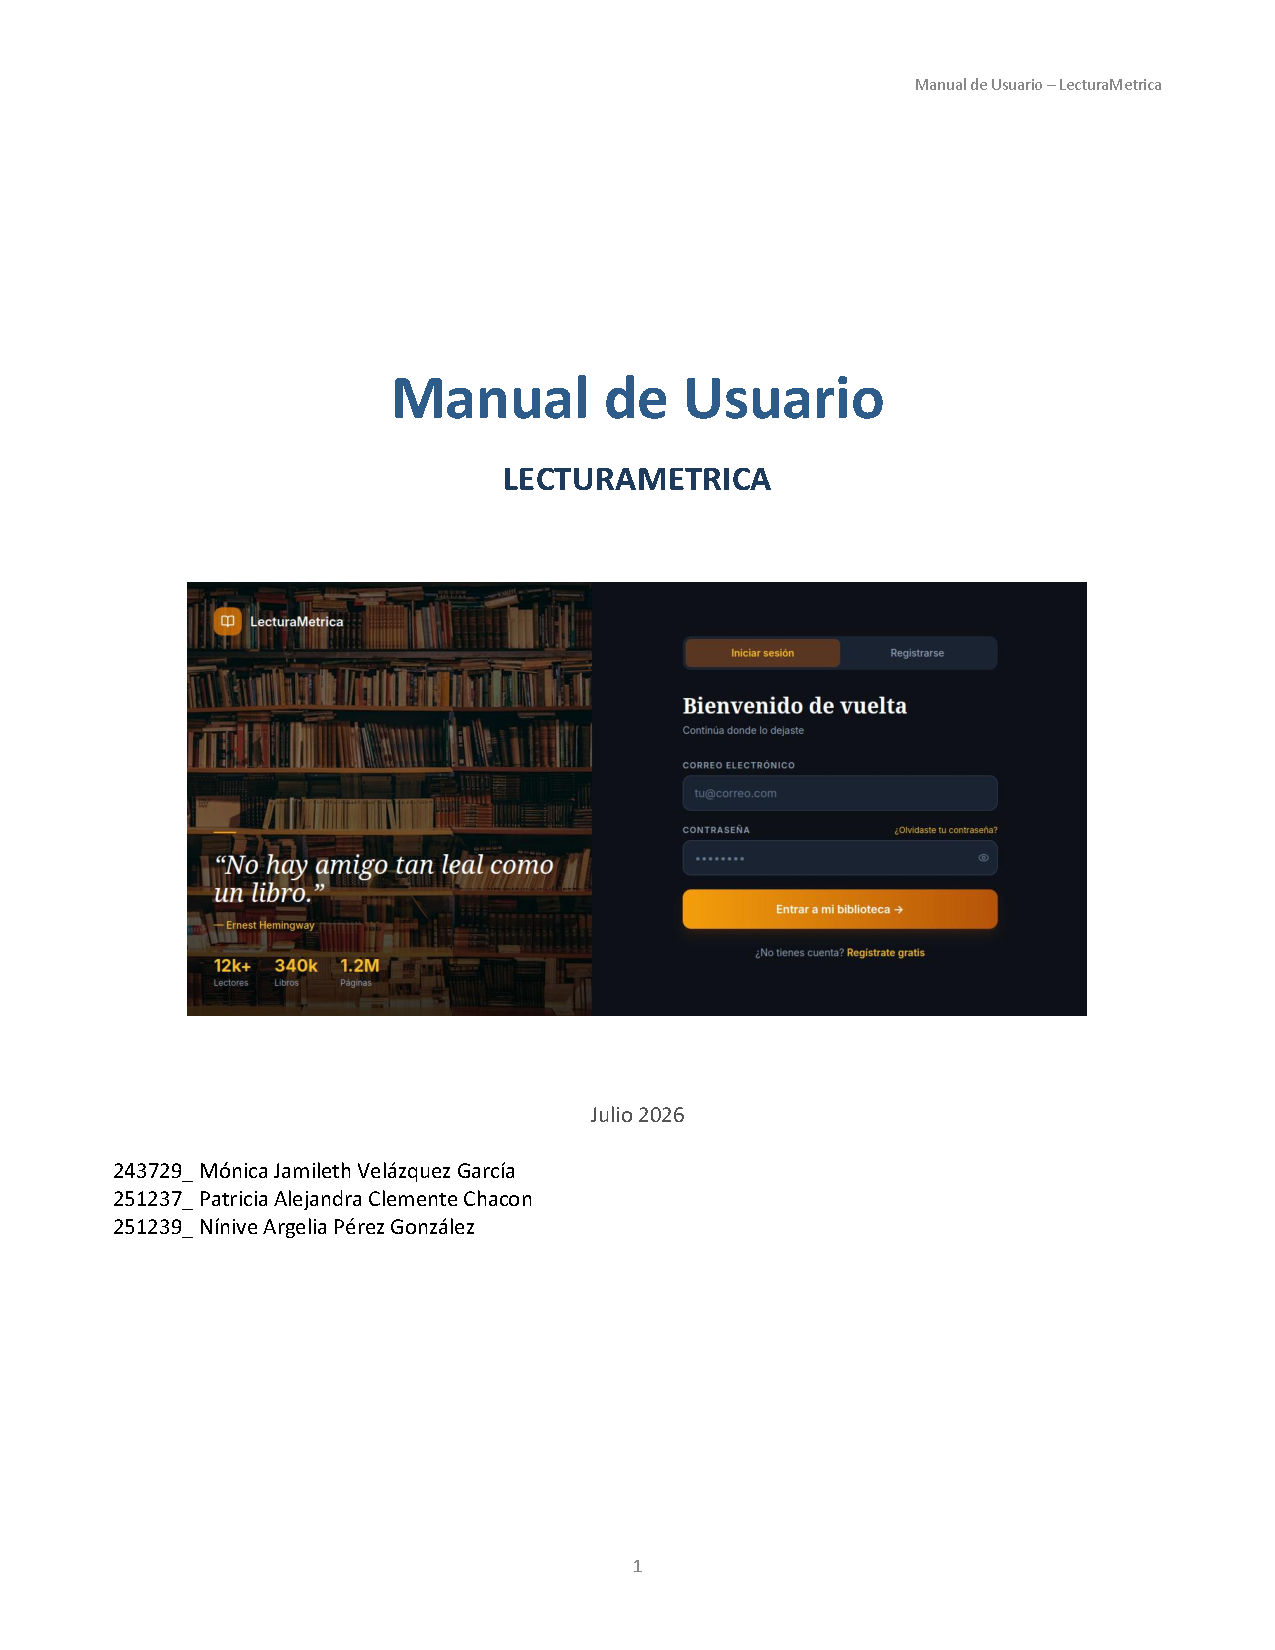
\includepdf[pages=-]{./anexos/Manual_de_Usuario.pdf}

% --- ANEXO 2: Casos de Uso ---
% Introducción al anexo para que no se vea puesto de golpe
\subsection*{Anexo B: Especificación y Narrativas de Casos de Uso}
\addcontentsline{toc}{subsection}{Anexo B: Especificación y Narrativas de Casos de Uso} % <-- ESTO TAMBIÉN
El presente anexo contiene la documentación detallada de las narrativas de casos de uso, flujos principales y flujos de excepción del sistema \textbf{LecturaMétrica}, elaborados como parte del análisis y diseño arquitectónico de la plataforma.

\vspace{0.5cm}

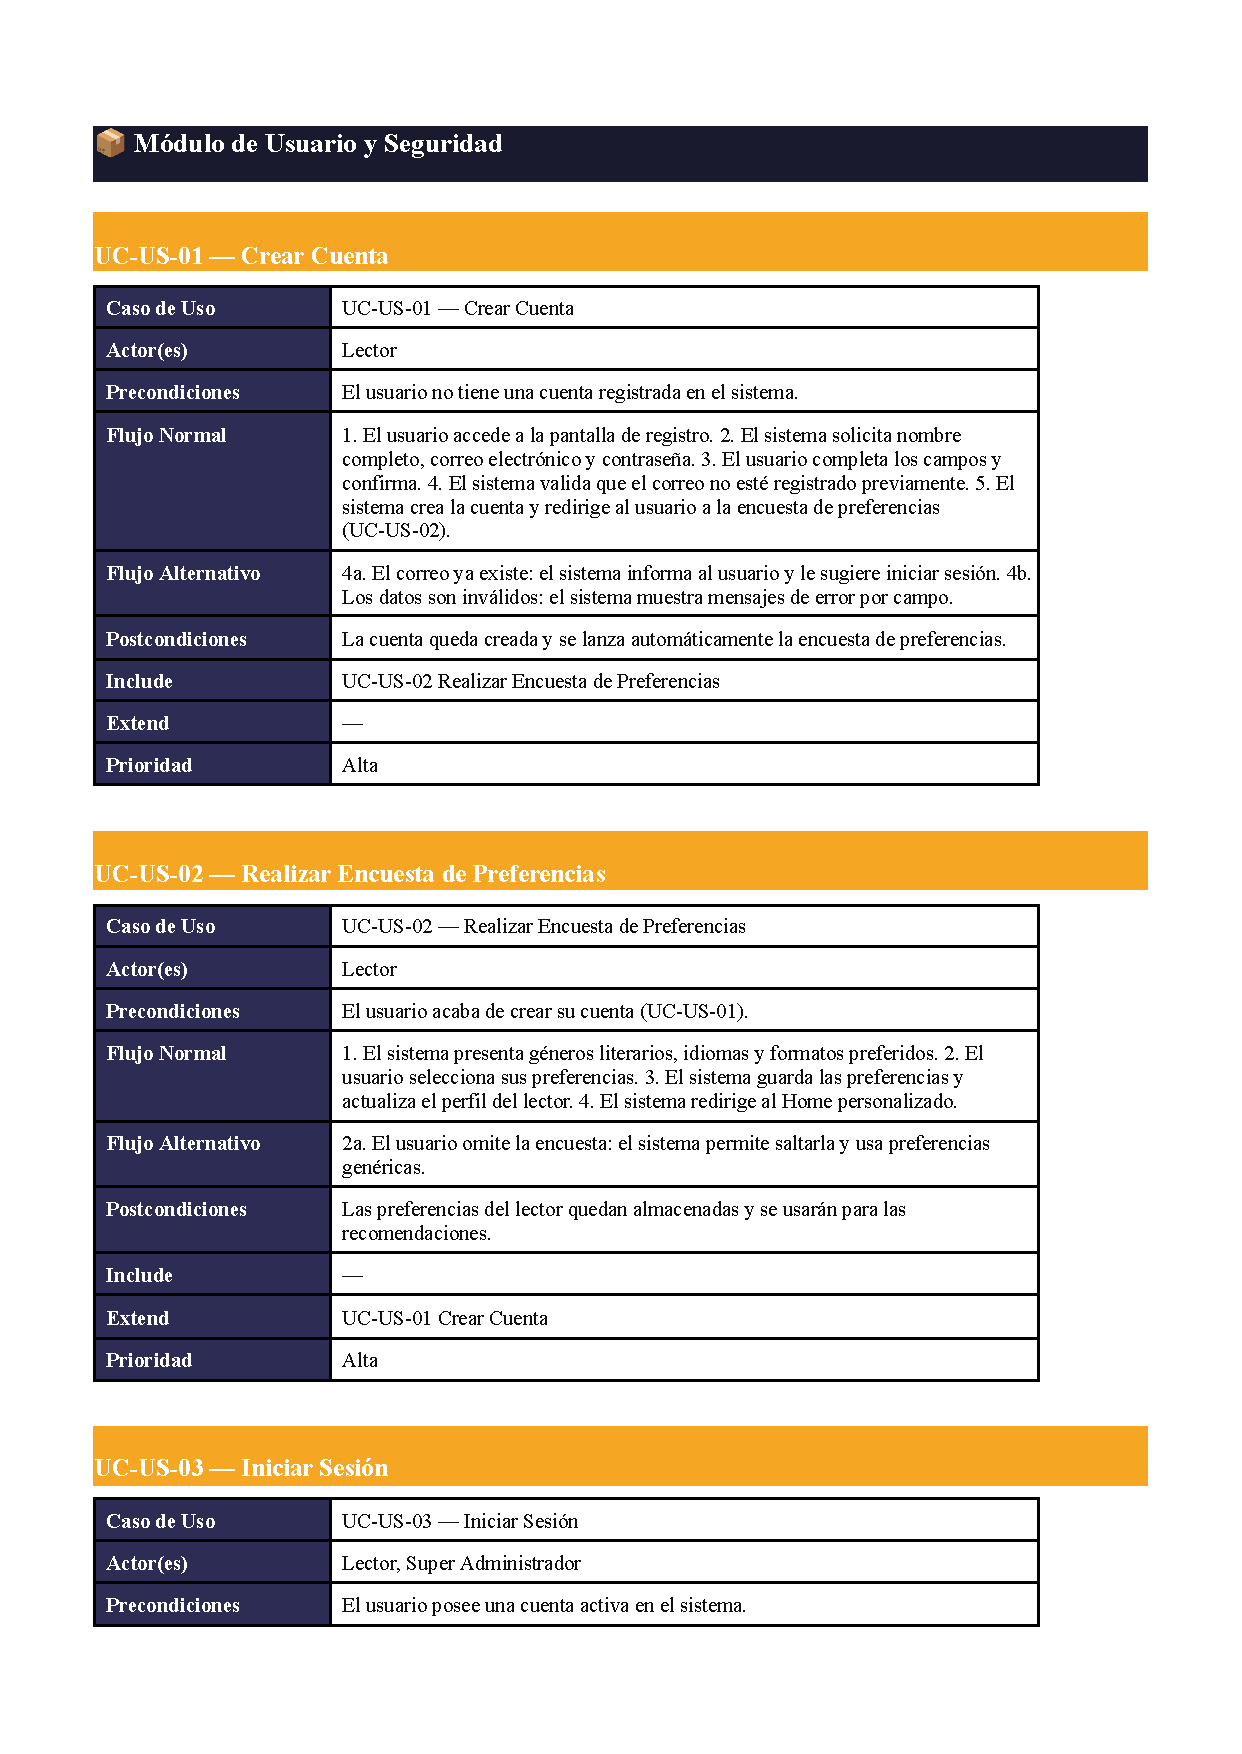
\includepdf[
    pages=-, 
    scale=0.90, 
    pagecommand={\thispagestyle{plain}}
]{./anexos/casos_de_uso_lecturametrica.docx.pdf}

% --- ANEXO 3: Diccionario de Datos de la Base de Datos ---
\subsection*{Anexo C: Diccionario de Datos del Sistema Relacional}
\addcontentsline{toc}{subsection}{Anexo C: Diccionario de Datos del Sistema Relacional}

El presente anexo contiene la especificación técnica exhaustiva de las 22 tablas que conforman el esquema relacional de la base de datos \textbf{LecturaMétrica} en PostgreSQL. Se detallan los nombres de atributos, tipos de datos nativos, llaves primarias (PK), llaves foráneas (FK), reglas de unicidad y descripciones funcionales para cada entidad del sistema:

\vspace{0.3cm}

\paragraph{1. Tabla: \texttt{users}}
\begin{table}[H]
	\centering
	\begin{tabular}{|l|l|l|p{6.5cm}|}
		\hline
		\textbf{Atributo} & \textbf{Tipo de Dato} & \textbf{Llave} & \textbf{Descripción / Restricción} \\ \hline
		id & UUID & PK & Identificador único del usuario. \\ \hline
		name & VARCHAR & - & Nombre del usuario. \\ \hline
		lastname & VARCHAR & - & Apellido del usuario. \\ \hline
		email & VARCHAR & UNIQUE & Correo electrónico único. \\ \hline
		password & VARCHAR & - & Hash de la contraseña. \\ \hline
		annual\_goal & INT4 & - & Meta anual de lectura. \\ \hline
		picture\_id & INT8 & FK & Referencia a \texttt{pictures(id)}. \\ \hline
		role\_id & UUID & FK & Referencia a \texttt{roles(id)}. \\ \hline
		deleted & BOOL & - & Estado de borrado lógico. \\ \hline
		deleted\_at & TIMESTAMP & - & Fecha/hora de eliminación lógica. \\ \hline
	\end{tabular}
	\caption{Esquema de la tabla \texttt{users}.}
\end{table}

\paragraph{2. Tabla: \texttt{roles}}
\begin{table}[H]
	\centering
	\begin{tabular}{|l|l|l|p{6.5cm}|}
		\hline
		\textbf{Atributo} & \textbf{Tipo de Dato} & \textbf{Llave} & \textbf{Descripción / Restricción} \\ \hline
		id & UUID & PK & Identificador único del rol. \\ \hline
		name & VARCHAR & - & Nombre del rol (ej. Lector, Admin). \\ \hline
	\end{tabular}
	\caption{Esquema de la tabla \texttt{roles}.}
\end{table}

\paragraph{3. Tabla: \texttt{books}}
\begin{table}[H]
	\centering
	\begin{tabular}{|l|l|l|p{6.5cm}|}
		\hline
		\textbf{Atributo} & \textbf{Tipo de Dato} & \textbf{Llave} & \textbf{Descripción / Restricción} \\ \hline
		id & UUID & PK & Identificador único de la obra. \\ \hline
		title & VARCHAR & - & Título del libro. \\ \hline
		isbn & VARCHAR & - & Código de identificación ISBN. \\ \hline
		cover & VARCHAR & - & URL o ruta de la portada. \\ \hline
		created\_at & TIMESTAMP & - & Fecha de creación. \\ \hline
		updated\_at & TIMESTAMP & - & Fecha de actualización. \\ \hline
		deleted & BOOL & - & Borrado lógico. \\ \hline
		deleted\_at & TIMESTAMP & - & Fecha de eliminación lógica. \\ \hline
	\end{tabular}
	\caption{Esquema de la tabla \texttt{books}.}
\end{table}

\paragraph{4. Tabla: \texttt{authors}}
\begin{table}[H]
	\centering
	\begin{tabular}{|l|l|l|p{6.5cm}|}
		\hline
		\textbf{Atributo} & \textbf{Tipo de Dato} & \textbf{Llave} & \textbf{Descripción / Restricción} \\ \hline
		id & INT8 & PK & Identificador único del autor. \\ \hline
		name & VARCHAR & - & Nombre completo del autor. \\ \hline
		description & VARCHAR & - & Biografía breve. \\ \hline
		created\_at & TIMESTAMP & - & Fecha de creación. \\ \hline
		updated\_at & TIMESTAMP & - & Fecha de actualización. \\ \hline
		deleted & BOOL & - & Borrado lógico. \\ \hline
		deleted\_at & TIMESTAMP & - & Fecha de eliminación lógica. \\ \hline
	\end{tabular}
	\caption{Esquema de la tabla \texttt{authors}.}
\end{table}

\paragraph{5. Tabla: \texttt{book\_authors}}
\begin{table}[H]
	\centering
	\begin{tabular}{|l|l|l|p{6.5cm}|}
		\hline
		\textbf{Atributo} & \textbf{Tipo de Dato} & \textbf{Llave} & \textbf{Descripción / Restricción} \\ \hline
		book\_id & UUID & PK, FK & Referencia a \texttt{books(id)}. \\ \hline
		author\_id & INT8 & PK, FK & Referencia a \texttt{authors(id)}. \\ \hline
	\end{tabular}
	\caption{Esquema de la tabla intermedia \texttt{book\_authors}.}
\end{table}

\paragraph{6. Tabla: \texttt{genders}}
\begin{table}[H]
	\centering
	\begin{tabular}{|l|l|l|p{6.5cm}|}
		\hline
		\textbf{Atributo} & \textbf{Tipo de Dato} & \textbf{Llave} & \textbf{Descripción / Restricción} \\ \hline
		id & INT8 & PK & Identificador del género. \\ \hline
		name & VARCHAR & - & Nombre del género literario. \\ \hline
		description & VARCHAR & - & Descripción del género. \\ \hline
		created\_at & TIMESTAMP & - & Fecha de creación. \\ \hline
		updated\_at & TIMESTAMP & - & Fecha de actualización. \\ \hline
		deleted & BOOL & - & Borrado lógico. \\ \hline
		deleted\_at & TIMESTAMP & - & Fecha de eliminación lógica. \\ \hline
	\end{tabular}
	\caption{Esquema de la tabla \texttt{genders}.}
\end{table}

\paragraph{7. Tabla: \texttt{book\_genres}}
\begin{table}[H]
	\centering
	\begin{tabular}{|l|l|l|p{6.5cm}|}
		\hline
		\textbf{Atributo} & \textbf{Tipo de Dato} & \textbf{Llave} & \textbf{Descripción / Restricción} \\ \hline
		book\_id & UUID & PK, FK & Referencia a \texttt{books(id)}. \\ \hline
		gender\_id & INT8 & PK, FK & Referencia a \texttt{genders(id)}. \\ \hline
	\end{tabular}
	\caption{Esquema de la tabla intermedia \texttt{book\_genres}.}
\end{table}

\paragraph{8. Tabla: \texttt{formats}}
\begin{table}[H]
	\centering
	\begin{tabular}{|l|l|l|p{6.5cm}|}
		\hline
		\textbf{Atributo} & \textbf{Tipo de Dato} & \textbf{Llave} & \textbf{Descripción / Restricción} \\ \hline
		id & INT8 & PK & Identificador único del formato. \\ \hline
		name & VARCHAR & - & Nombre del formato (físico, digital, etc.). \\ \hline
		description & VARCHAR & - & Descripción del formato. \\ \hline
	\end{tabular}
	\caption{Esquema de la tabla \texttt{formats}.}
\end{table}

\paragraph{9. Tabla: \texttt{reading\_status}}
\begin{table}[H]
	\centering
	\begin{tabular}{|l|l|l|p{6.5cm}|}
		\hline
		\textbf{Atributo} & \textbf{Tipo de Dato} & \textbf{Llave} & \textbf{Descripción / Restricción} \\ \hline
		id & INT8 & PK & Identificador del estado de lectura. \\ \hline
		name & VARCHAR & - & Nombre del estado (ej. leyendo, por leer). \\ \hline
		description & VARCHAR & - & Descripción breve del estado. \\ \hline
		created\_at & TIMESTAMP & - & Fecha de creación. \\ \hline
		updated\_at & TIMESTAMP & - & Fecha de actualización. \\ \hline
		deleted & BOOL & - & Borrado lógico. \\ \hline
		deleted\_at & TIMESTAMP & - & Fecha de eliminación lógica. \\ \hline
	\end{tabular}
	\caption{Esquema de la tabla \texttt{reading\_status}.}
\end{table}

\paragraph{10. Tabla: \texttt{user\_library}}
\begin{table}[H]
	\centering
	\begin{tabular}{|l|l|l|p{6.5cm}|}
		\hline
		\textbf{Atributo} & \textbf{Tipo de Dato} & \textbf{Llave} & \textbf{Descripción / Restricción} \\ \hline
		id & UUID & PK & Identificador único del registro. \\ \hline
		user\_id & UUID & FK & Referencia a \texttt{users(id)}. \\ \hline
		book\_id & UUID & FK & Referencia a \texttt{books(id)}. \\ \hline
		format\_id & INT8 & FK & Referencia a \texttt{formats(id)}. \\ \hline
		reading\_status\_id & INT8 & FK & Referencia a \texttt{reading\_status(id)}. \\ \hline
		current\_page & INT4 & - & Página actual. \\ \hline
		total\_page & INT4 & - & Total de páginas del libro. \\ \hline
		current\_chapter & INT4 & - & Capítulo actual. \\ \hline
		total\_chapter & INT4 & - & Total de capítulos. \\ \hline
		is\_favorite & BOOL & - & Indicador de favorito. \\ \hline
		finished\_at & DATE & - & Fecha en que se finalizó. \\ \hline
	\end{tabular}
	\caption{Esquema de la tabla \texttt{user\_library}.}
\end{table}

\paragraph{11. Tabla: \texttt{library\_notes}}
\begin{table}[H]
	\centering
	\begin{tabular}{|l|l|l|p{6.5cm}|}
		\hline
		\textbf{Atributo} & \textbf{Tipo de Dato} & \textbf{Llave} & \textbf{Descripción / Restricción} \\ \hline
		id & INT8 & PK & Identificador de la nota. \\ \hline
		user\_library\_id & UUID & FK & Referencia a \texttt{user\_library(id)}. \\ \hline
		chapter & INT4 & - & Capítulo referenciado. \\ \hline
		page & INT4 & - & Página referenciada. \\ \hline
		content & TEXT & - & Contenido de la nota. \\ \hline
		created\_at & TIMESTAMP & - & Fecha de creación. \\ \hline
	\end{tabular}
	\caption{Esquema de la tabla \texttt{library\_notes}.}
\end{table}

\paragraph{12. Tabla: \texttt{reading\_sessions}}
\begin{table}[H]
	\centering
	\begin{tabular}{|l|l|l|p{6.5cm}|}
		\hline
		\textbf{Atributo} & \textbf{Tipo de Dato} & \textbf{Llave} & \textbf{Descripción / Restricción} \\ \hline
		id & UUID & PK & Identificador de la sesión de lectura. \\ \hline
		user\_library\_id & UUID & FK & Referencia a \texttt{user\_library(id)}. \\ \hline
		pages\_read & INT4 & - & Páginas leídas en la sesión. \\ \hline
		chapters\_read & INT4 & - & Capítulos leídos en la sesión. \\ \hline
		seconds\_read & INT4 & - & Duración en segundos. \\ \hline
		date & DATE & - & Fecha de la sesión. \\ \hline
		is\_flagged & BOOL & - & Indicador de anomalía/alerta. \\ \hline
		flag\_reason & VARCHAR & - & Motivo del reporte/alerta. \\ \hline
	\end{tabular}
	\caption{Esquema de la tabla \texttt{reading\_sessions}.}
\end{table}

\paragraph{13. Tabla: \texttt{badges}}
\begin{table}[H]
	\centering
	\begin{tabular}{|l|l|l|p{6.5cm}|}
		\hline
		\textbf{Atributo} & \textbf{Tipo de Dato} & \textbf{Llave} & \textbf{Descripción / Restricción} \\ \hline
		id & INT8 & PK & Identificador de la insignia. \\ \hline
		name & VARCHAR & - & Nombre del logro/insignia. \\ \hline
		description & VARCHAR & - & Descripción de la insignia. \\ \hline
		public\_id & VARCHAR & - & ID público del recurso gráfico. \\ \hline
		url & VARCHAR & - & URL de la imagen de la insignia. \\ \hline
		created\_at & TIMESTAMP & - & Fecha de creación. \\ \hline
		updated\_at & TIMESTAMP & - & Fecha de actualización. \\ \hline
		deleted & BOOL & - & Borrado lógico. \\ \hline
		deleted\_at & TIMESTAMP & - & Fecha de eliminación lógica. \\ \hline
	\end{tabular}
	\caption{Esquema de la tabla \texttt{badges}.}
\end{table}

\paragraph{14. Tabla: \texttt{user\_badges}}
\begin{table}[H]
	\centering
	\begin{tabular}{|l|l|l|p{6.5cm}|}
		\hline
		\textbf{Atributo} & \textbf{Tipo de Dato} & \textbf{Llave} & \textbf{Descripción / Restricción} \\ \hline
		id & INT8 & PK & Identificador del registro. \\ \hline
		user\_id & UUID & FK & Referencia a \texttt{users(id)}. \\ \hline
		badge\_id & INT8 & FK & Referencia a \texttt{badges(id)}. \\ \hline
		created\_at & TIMESTAMP & - & Fecha en que se obtuvo la insignia. \\ \hline
	\end{tabular}
	\caption{Esquema de la tabla \texttt{user\_badges}.}
\end{table}

\paragraph{15. Tabla: \texttt{user\_streaks}}
\begin{table}[H]
	\centering
	\begin{tabular}{|l|l|l|p{6.5cm}|}
		\hline
		\textbf{Atributo} & \textbf{Tipo de Dato} & \textbf{Llave} & \textbf{Descripción / Restricción} \\ \hline
		id & UUID & PK & Identificador de la racha. \\ \hline
		user\_id & UUID & FK & Referencia a \texttt{users(id)}. \\ \hline
		current\_streak & INT4 & - & Racha actual de días consecutivos. \\ \hline
		max\_streak & INT4 & - & Racha máxima alcanzada. \\ \hline
		last\_activity\_date & DATE & - & Fecha de última actividad registrada. \\ \hline
	\end{tabular}
	\caption{Esquema de la tabla \texttt{user\_streaks}.}
\end{table}

\paragraph{16. Tabla: \texttt{user\_pref\_formats}}
\begin{table}[H]
	\centering
	\begin{tabular}{|l|l|l|p{6.5cm}|}
		\hline
		\textbf{Atributo} & \textbf{Tipo de Dato} & \textbf{Llave} & \textbf{Descripción / Restricción} \\ \hline
		user\_preference\_id & UUID & PK, FK & Identificador de preferencia. \\ \hline
		formats\_id & INT8 & PK, FK & Referencia a \texttt{formats(id)}. \\ \hline
	\end{tabular}
	\caption{Esquema de la tabla \texttt{user\_pref\_formats}.}
\end{table}

\paragraph{17. Tabla: \texttt{user\_pref\_genres}}
\begin{table}[H]
	\centering
	\begin{tabular}{|l|l|l|p{6.5cm}|}
		\hline
		\textbf{Atributo} & \textbf{Tipo de Dato} & \textbf{Llave} & \textbf{Descripción / Restricción} \\ \hline
		user\_preference\_id & UUID & PK, FK & Identificador de preferencia. \\ \hline
		genres\_id & INT8 & PK, FK & Referencia a \texttt{genders(id)}. \\ \hline
	\end{tabular}
	\caption{Esquema de la tabla \texttt{user\_pref\_genres}.}
\end{table}

\paragraph{18. Tabla: \texttt{recommendations}}
\begin{table}[H]
	\centering
	\begin{tabular}{|l|l|l|p{6.5cm}|}
		\hline
		\textbf{Atributo} & \textbf{Tipo de Dato} & \textbf{Llave} & \textbf{Descripción / Restricción} \\ \hline
		id & UUID & PK & Identificador de la recomendación. \\ \hline
		user\_id & UUID & FK & Referencia a \texttt{users(id)}. \\ \hline
	\end{tabular}
	\caption{Esquema de la tabla \texttt{recommendations}.}
\end{table}

\paragraph{19. Tabla: \texttt{recommendation\_contents}}
\begin{table}[H]
	\centering
	\begin{tabular}{|l|l|l|p{6.5cm}|}
		\hline
		\textbf{Atributo} & \textbf{Tipo de Dato} & \textbf{Llave} & \textbf{Descripción / Restricción} \\ \hline
		id & INT8 & PK & Identificador del contenido. \\ \hline
		content & VARCHAR & - & Texto del contenido. \\ \hline
		sender\_id & UUID & FK & Referencia al remitente \texttt{users(id)}. \\ \hline
		book\_id & UUID & FK & Referencia a \texttt{books(id)}. \\ \hline
	\end{tabular}
	\caption{Esquema de la tabla \texttt{recommendation\_contents}.}
\end{table}

\paragraph{20. Tabla: \texttt{letters}}
\begin{table}[H]
	\centering
	\begin{tabular}{|l|l|l|p{6.5cm}|}
		\hline
		\textbf{Atributo} & \textbf{Tipo de Dato} & \textbf{Llave} & \textbf{Descripción / Restricción} \\ \hline
		id & INT8 & PK & Identificador de la carta. \\ \hline
		receiver\_id & UUID & FK & Referencia al destinatario \texttt{users(id)}. \\ \hline
		recommendation\_content\_id & INT8 & FK & Referencia a \texttt{recommendation\_contents(id)}. \\ \hline
		claimed\_at & TIMESTAMP & - & Fecha de reclamo o recepción. \\ \hline
	\end{tabular}
	\caption{Esquema de la tabla \texttt{letters}.}
\end{table}

\paragraph{21. Tabla: \texttt{curiosities}}
\begin{table}[H]
	\centering
	\begin{tabular}{|l|l|l|p{6.5cm}|}
		\hline
		\textbf{Atributo} & \textbf{Tipo de Dato} & \textbf{Llave} & \textbf{Descripción / Restricción} \\ \hline
		id & INT8 & PK & Identificador de la curiosidad. \\ \hline
		title & VARCHAR & - & Título del dato curioso. \\ \hline
		fact & TEXT & - & Explicación o hecho curioso. \\ \hline
		genre & VARCHAR & - & Género asociado. \\ \hline
		book\_reference & VARCHAR & - & Referencia al libro. \\ \hline
	\end{tabular}
	\caption{Esquema de la tabla \texttt{curiosities}.}
\end{table}

\paragraph{22. Tabla: \texttt{pictures}}
\begin{table}[H]
	\centering
	\begin{tabular}{|l|l|l|p{6.5cm}|}
		\hline
		\textbf{Atributo} & \textbf{Tipo de Dato} & \textbf{Llave} & \textbf{Descripción / Restricción} \\ \hline
		id & INT8 & PK & Identificador de la imagen. \\ \hline
		name & VARCHAR & - & Nombre del archivo. \\ \hline
		description & VARCHAR & - & Descripción de la imagen. \\ \hline
		public\_id & VARCHAR & - & Identificador público del hosting. \\ \hline
		url & VARCHAR & - & Enlace directo a la imagen. \\ \hline
		created\_at & TIMESTAMP & - & Fecha de creación. \\ \hline
		updated\_at & TIMESTAMP & - & Fecha de actualización. \\ \hline
		deleted & BOOL & - & Borrado lógico. \\ \hline
		deleted\_at & TIMESTAMP & - & Fecha de eliminación lógica. \\ \hline
	\end{tabular}
	\caption{Esquema de la tabla \texttt{pictures}.}
\end{table}

\end{document}

